% Options for packages loaded elsewhere
\PassOptionsToPackage{unicode}{hyperref}
\PassOptionsToPackage{hyphens}{url}
\documentclass[
]{article}
\usepackage{xcolor}
\usepackage{amsmath,amssymb}
\setcounter{secnumdepth}{-\maxdimen} % remove section numbering
\usepackage{iftex}
\ifPDFTeX
  \usepackage[T1]{fontenc}
  \usepackage[utf8]{inputenc}
  \usepackage{textcomp} % provide euro and other symbols
\else % if luatex or xetex
  \usepackage{unicode-math} % this also loads fontspec
  \defaultfontfeatures{Scale=MatchLowercase}
  \defaultfontfeatures[\rmfamily]{Ligatures=TeX,Scale=1}
\fi
\usepackage{lmodern}
\ifPDFTeX\else
  \setmainfont{Times New Roman}
  \setmathfont{STIX Two Math}
\fi
\usepackage[margin=1in]{geometry}
\usepackage{setspace}
\usepackage{lineno}
\renewcommand\linenumberfont{\normalfont\scriptsize}
\ifPDFTeX\else
  % xetex/luatex font selection
\fi
% Use upquote if available, for straight quotes in verbatim environments
\IfFileExists{upquote.sty}{\usepackage{upquote}}{}
\IfFileExists{microtype.sty}{% use microtype if available
  \usepackage[]{microtype}
  \UseMicrotypeSet[protrusion]{basicmath} % disable protrusion for tt fonts
}{}
\makeatletter
\@ifundefined{KOMAClassName}{% if non-KOMA class
  \IfFileExists{parskip.sty}{%
    \usepackage{parskip}
  }{% else
    \setlength{\parindent}{0pt}
    \setlength{\parskip}{6pt plus 2pt minus 1pt}}
}{% if KOMA class
  \KOMAoptions{parskip=half}}
\makeatother
\usepackage{longtable,booktabs,array}
\setlength\LTleft{0pt plus 1fill}
\setlength\LTright{0pt plus 1fill}
\newcounter{none} % for unnumbered tables
\usepackage{calc} % for calculating minipage widths
% Correct order of tables after \paragraph or \subparagraph
\usepackage{etoolbox}
\makeatletter
\patchcmd\longtable{\par}{\if@noskipsec\mbox{}\fi\par}{}{}
\makeatother
% Allow footnotes in longtable head/foot
\IfFileExists{footnotehyper.sty}{\usepackage{footnotehyper}}{\usepackage{footnote}}
\makesavenoteenv{longtable}
\usepackage{graphicx}
\usepackage{float}
\makeatletter
\newsavebox\pandoc@box
\newcommand*\pandocbounded[1]{% scales image to fit in text height/width
  \sbox\pandoc@box{#1}%
  \Gscale@div\@tempa{\textheight}{\dimexpr\ht\pandoc@box+\dp\pandoc@box\relax}%
  \Gscale@div\@tempb{\linewidth}{\wd\pandoc@box}%
  \ifdim\@tempb\p@<\@tempa\p@\let\@tempa\@tempb\fi% select the smaller of both
  \ifdim\@tempa\p@<\p@\scalebox{\@tempa}{\usebox\pandoc@box}%
  \else\usebox{\pandoc@box}%
  \fi%
}
% Set default figure placement to htbp
\def\fps@figure{htbp}
\makeatother
\ifLuaTeX
  \usepackage{luacolor}
  \usepackage[soul]{lua-ul}
\else
  \usepackage{soul}
\fi
\setlength{\emergencystretch}{3em} % prevent overfull lines
\providecommand{\tightlist}{%
  \setlength{\itemsep}{0pt}\setlength{\parskip}{0pt}}
\usepackage{bookmark}
\IfFileExists{xurl.sty}{\usepackage{xurl}}{} % add URL line breaks if available
\urlstyle{same}
\hypersetup{
  pdftitle={Spore-informed agroclimatic modelling improves the timing of grapevine downy mildew management in subtropical vineyards},
  hidelinks,
  pdfcreator={LaTeX via pandoc}}

\title{Spore-informed agroclimatic modelling improves the timing of
grapevine downy mildew management in subtropical vineyards}
\author{}
\date{}

\begin{document}
\doublespacing
\pagenumbering{arabic}
\linenumbers
\maketitle

Linjia Yao \textsuperscript{a \#}, Bin Chen \textsuperscript{b \#},
Vittorio Rossi \textsuperscript{c}, Ling Yin \textsuperscript{d}, Shumei
Wei \textsuperscript{d}, Qi Tian \textsuperscript{a}, Changqing Yan
\textsuperscript{e}, Hui wang \textsuperscript{f}, Antonio Fernandes
Nogueira Júnior \textsuperscript{g}, Yu Huang \textsuperscript{h}, Qiang
Yu \textsuperscript{b *}, Junjie Qu \textsuperscript{d *}, Gang Zhao
\textsuperscript{b *}

\textsuperscript{a} College of Natural Resources and Environment,
Northwest A \& F University, Yangling 712100, China

\textsuperscript{b} State Key Laboratory of Soil and Water Conservation
and Desertification Control, College of Soil and Water Conservation
Science and Engineering, Northwest A\&F University, Yangling, Shaanxi
712100, China

\textsuperscript{c} Research centre on Plant Health Modelling (PHEM),
Università Cattolica del Sacro Cuore, Piacenza, Italy

\textsuperscript{d} Guangxi Crop Genetic Improvement and Biotechnology
Key Lab, Guangxi Academy of Agricultural Sciences, Nanning 530007, China

\textsuperscript{e} College of Intelligent Equipment, Shandong
University of Science and Technology, Taian 271019, China

\textsuperscript{f} Institute of Plant Protection Beijing Academy of
Agriculture and Forestry Sciences, 100097 Beijing, China

\textsuperscript{g} KWS SAAT SE \& Co. KGaA, Einbeck, Germany

\textsuperscript{h} Grape and Wine Research Institute, Guangxi Academy
of Agricultural Sciences, Nanning, Guangxi 530007, China

\textbf{* Corresponding author:} Prof. Qiang Yu, E-mail:
\href{mailto:yuq@nwafu.edu.cn}{\nolinkurl{yuq@nwafu.edu.cn}}; Prof.
Junjie Qu, E-mail:
\href{mailto:qujunjie@gxaas.net}{\nolinkurl{qujunjie@gxaas.net}}; Prof.
Gang Zhao, E-mail: gang.zhao@nwafu.edu.cn

\textbf{\textsuperscript{\#} These authors contributed equally to this
work.}

\section{Abstract}\label{abstract}

Calendar-based fungicide programmes remain common in humid subtropical
vineyards, where warm and wet conditions favour grapevine downy mildew
(\emph{Plasmopara viticola}) and make the timing of early-season
protection difficult. Existing mechanistic warning models were largely
developed for oospore-driven primary infections in temperate systems,
whereas first seasonal infections in subtropical vineyards may be driven
by continuously available asexual sporangia. To support field-based
disease management, we developed a spore-informed agroclimatic modelling
framework for predicting first seasonal infection under subtropical
conditions. The framework integrates primary and secondary infection
processes into a First Seasonal Infection Model (FSIM) and extends it by
incorporating field-observed sporangia through a dynamic spore-pressure
field that regulates infection triggering (FSIM-S). Model calibration
and validation using three-year, multi-site observations from two
commercial vineyards and one experimental orchard in Guangxi, China
(2022--2024) showed that FSIM predicted
infection timing with a mean absolute error (MAE) of 9.3 days and a root
mean square error (RMSE) of 10.6 days. Incorporating spore pressure
reduced MAE and RMSE to 6.3 and 6.5 days, respectively. Regional
simulations for 2000--2024 identified a stable high-risk window around
DOY 180--210 and indicated that model-guided timing could avoid 2--5
early preventive fungicide applications per season relative to a
calendar-based programme. FSIM-S links airborne inoculum monitoring with
agroclimatic process modelling and provides a field-tested basis for
climate-smart, model-guided management of grapevine downy mildew in
subtropical viticulture.

\textbf{Key words:} Agroclimatic modelling, Spore-pressure dynamics,
Fungicide timing, Subtropical viticulture, Smart agriculture

\section{Introduction}\label{introduction}

Since 2000, China's grape industry has expanded rapidly, and humid
subtropical regions have become increasingly important production zones
(National Bureau of Statistics of China, 2024; Fig. S1). These
production systems are exposed to persistent crop-protection pressure
because warm, humid and rainfall-prone conditions frequently coincide
with early grapevine development, when young leaves and inflorescences
are highly susceptible to grapevine downy mildew (GDM), caused by
\emph{Plasmopara viticola}. Severe epidemics impair canopy
photosynthetic capacity and induce flower and fruit rotting and
abscission, with yield losses exceeding 75\% in epidemic years (Nogueira
Júnior et al., 2019; Mouafo-Tchinda et al., 2022; Koledenkova et al.,
2022; Peng et al., 2024). Consequently, disease management in many
vineyards still relies heavily on experience-based and calendar-driven
preventive spraying, often involving 8--12 fungicide applications per
growing season (García-Esparza et al., 2006). Although such programmes
can protect yield, their limited responsiveness to local infection risk
may increase production costs, pesticide selection pressure and
environmental burdens (Yin et al., 2023).

More accurate identification of the first seasonal infection window is
therefore central to risk-based disease management in subtropical
viticulture. Previous studies have shown that adapting grape downy
mildew control to local onset risk can reduce unnecessary fungicide
treatments (Chen et al., 2019, 2020), but reliable early-season timing
remains difficult where favourable weather, host susceptibility and
viable inoculum do not necessarily coincide. Early forecasting
approaches were largely empirical and relied on weather thresholds, such
as the ``3--10 rule'' (Baldacci, 1947) and the EPI (État Potentiel
d'Infection) model (Strizyk, 1983), which use combinations of
meteorological conditions to indicate infection risk (Caffi et al.,
2007). These approaches are operationally simple,
but their limited representation of spore production, dispersal and
infection processes reduces their transferability across contrasting
climatic regions. Semi-mechanistic models subsequently improved the
biological representation of spore development and dispersal (Hill,
1990; Puelles et al., 2024), yet many remain tied to specific assumptions
about initial inoculum sources, pathogen phenology or local climatic
contexts.

The mechanistic Rossi model (RM) represents a major advance for
temperate vineyards, where overwintered oospores constitute the primary
source of early-season inoculum (Gobbin et al., 2005; Rossi et al.,
2008). RM explicitly describes the oospore-driven primary infection
pathway from oospore maturation and germination to sporangia formation,
zoospore release, dispersal, infection and symptom expression, while
coupling these biological stages with temperature, rainfall, relative
humidity and leaf wetness. Field applications have shown that RM-based
forecasts can improve the timing of early disease control and reduce
seasonal spray numbers without compromising protection (Caffi et al.,
2010). As a result, RM has become a benchmark framework for
mechanistic primary infection forecasting in temperate grape production
systems.

Tropical and subtropical viticultural systems differ markedly from these
temperate settings in both climatic seasonality and pathogen survival
ecology (Carisse, 2016; Yi et al., 2019; Yu et al., 2022; Kocsis et
al., 2024). In regions with mild winters, variable pruning-induced
growth cycles or extended periods of green tissue availability,
\emph{P. viticola} may persist through asexual pathways rather than
being reintroduced each season through oospore-driven primary infection
(Hug, 2005; Gobbin et al., 2006; Rumbou and Gessler, 2006; Koopman et
al., 2007). In Sri Lanka, for example, evergreen grapevine production
cycles initiated by pruning are associated with epidemics apparently
triggered by sporangia produced on green vegetation, while oospores were
not observed despite targeted searches (Ramanathan and Sivapalan, 1988).
In subtropical Brazil, population genetic patterns indicated epidemics
dominated by clonal infections, consistent with predominantly asexual
reproduction. In other mild-winter regions, such as California and
Western Australia, the pathogen has been suggested to survive as
mycelium in buds and persistent leaves (Barrett, 1939; Killigrew et
al., 2005), although successful sporulation from lesions on lignified
canes has not been demonstrated (Taylor, 2018). Collectively, these
observations indicate that climate-dependent survival and inoculum
pathways can alter the biological basis of first seasonal infection.

This epidemiological divergence creates a modelling gap for subtropical
disease management. Mechanistic frameworks developed for oospore-driven
primary infection may not adequately represent systems in which
airborne asexual sporangia constitute a persistent or recurrent inoculum
source during early crop development. At the same time, airborne
sporangia monitoring has been shown to provide useful information for
disease prediction (Brischetto et al., 2021; Carisse et al., 2021), but
such observations have rarely been embedded within process-based models
as dynamic constraints on infection triggering. A field-tested framework
that jointly represents asexual inoculum pressure, meteorological
suitability and host susceptibility is therefore needed to support
climate-adaptive disease management in subtropical vineyards.

To address this need, we developed a \emph{First Seasonal Infection
Model} (FSIM) for tropical and subtropical viticultural conditions by
restructuring the epidemiological framework derived from the Rossi
primary infection model and related infection-risk approaches (Rossi et
al., 2008; Brischetto et al., 2021). In this study, first seasonal
infection denotes the earliest infection event of a new grape-growing
season driven by asexual inoculum, in contrast to oospore-driven primary
infection in temperate systems. Airborne asexual spores were treated as
the initial inoculum and coupled with key meteorological drivers to
simulate infection timing. Field sporangia observations were then
incorporated as a dynamic inoculum pressure field, producing an extended
model (FSIM-S) in which infection triggering is constrained by both
environmental suitability and observed spore pressure. The framework was
evaluated using three-year, multi-site field observations in Guangxi and
applied to regional disease reconstruction and model-guided management
scenario analysis. By linking inoculum monitoring with agroclimatic
process modelling, FSIM-S provides a basis for climate-smart grapevine
downy mildew management in subtropical viticulture.

\section{Materials and methods}\label{materials-and-methods}

\subsection{Study design and overall
workflow}\label{study-design-and-overall-workflow}

This study was designed as a three-year, multi-site, field-based
agronomic modelling study in two commercial vineyards and one
experimental orchard under subtropical conditions. The
workflow combined field observations, process-based modelling, and
regional simulation to characterize the mechanisms governing first
seasonal infection of grapevine downy mildew and to evaluate the
potential of the proposed framework for improving disease-management timing
(\hyperref[_Ref225433957]{Fig 1}). The overall design comprised three
main stages: (1) multi-site field monitoring to capture airborne
inoculum dynamics, grapevine phenology, management records, and the
timing of first seasonal infection; (2) development of a biologically
consistent \emph{First Seasonal Infection Model} (FSIM), followed by
stepwise evaluation, optimization, and calibration; and (3)
regional-scale simulations driven by long-term meteorological data to
assess infection risk and disease-management scenarios.

Field experiments were conducted from 2022 to 2024 in two commercial
vineyards and one experimental orchard located in Nanning, Guilin, and
Hechi, Guangxi Province.
Observations included: (i) continuous monitoring of airborne \emph{P. viticola}
inoculum, (ii) dates of first visible downy mildew lesions of the
season, which were used to determine first seasonal infection timing,
(iii) grapevine phenological stages, and (iv) agronomic management
records. Historical hourly meteorological data for the period 2000--2024
were obtained from the ERA5 reanalysis dataset and used to provide
meteorological forcing for model simulations (Hersbach et al., 2020).

At the modelling stage, the newly developed FSIM was first
systematically evaluated to examine its ability to represent the timing
of first seasonal infection under subtropical conditions in Guangxi.
Subsequently, field-based spore monitoring data were incorporated to
characterize inoculum pressure and to constrain infection processes,
resulting in an observation-informed framework (FSIM-S).

The models were parameterized and cross-validated using multi-site field
observations (2022--2024). The optimized framework was then applied in
regional simulations covering 2000--2024 to quantify long-term spatial
variability in infection risk and to assess the management implications
of model-informed decision support (Zhao et al., 2024).

\begin{figure}[H]
\centering
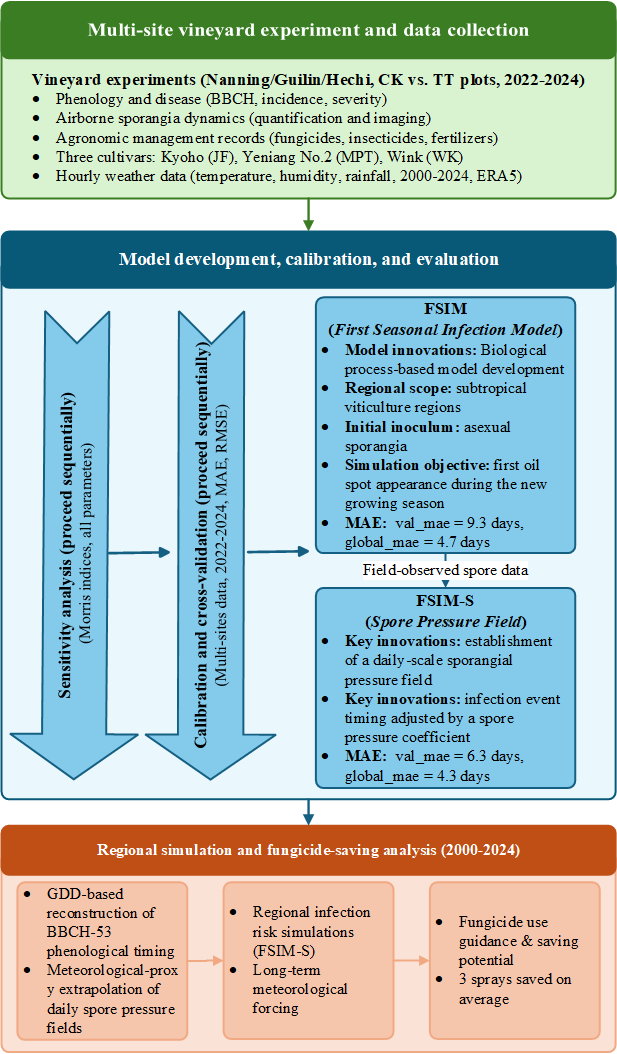
\includegraphics[width=0.65\linewidth]{fig/Figure_01.png}
\caption{Overall workflow of this study. CK indicates control plots
without fungicide applications, whereas TT denotes plots managed under
conventional fungicide schedules.}
\label{_Ref225433957}
\end{figure}

\subsection{Field experiments and data
collection}\label{field-experiments-and-data-collection}

\subsubsection{Site description, climate, vineyard
layout}\label{site-description-climate-vineyard-layout}

Field experiments were conducted from 2022 to 2024 in two commercial
vineyards and one experimental orchard located in the humid subtropical
zone of the Guangxi Zhuang Autonomous Region, southern China,
specifically in Xing'an (Guilin), Du'an (Hechi), and Jiangnan (Nanning)
(\hyperref[_Ref222580265]{Table 1}; \hyperref[_Ref212629919]{Fig
2a,b}). These sites span a pronounced
mesoscale gradient in thermal and moisture conditions and collectively
characterize the early-season climatic context of the study region. Over
the three-year study period, the mean air temperature across sites was
21.0 °C, and relative humidity remained persistently high (mean 75.9\%).
Rainfall was abundant and frequent, with a multi-year mean annual total
of 2,134 mm and an average of 149 rainy days per year. Rainy days were
defined as days with daily precipitation \textgreater0.2 mm, consistent
with the resolution of the meteorological dataset used
(\hyperref[_Ref214271335]{Fig 3}).

Compared with temperate viticultural regions of central Europe, winter
conditions at the study sites were characterized by relatively high
temperature and humidity and typically did not include severe cold
events (\hyperref[_Ref214271335]{Fig 3}). In addition, the adoption of a
secondary cropping system at some vineyards resulted in delayed leaf
senescence, with natural leaf fall extending into January--February in
certain years, while budburst of the subsequent growth cycle generally
occurred in March--April. As a consequence, the dormancy period was
short and phenologically discontinuous (\hyperref[_Ref222580265]{Table
1}).

To reflect representative grape production systems in southern China,
each experimental site was planted with a locally widespread and
commonly cultivated variety: `Wink' in Guilin, `Yeniang No. 2' in Hechi,
and `Kyoho' in Nanning. Detailed site characteristics, including
planting year, vine spacing, and cropping system (including the presence
or absence of secondary cropping), are summarized in
\hyperref[_Ref222580265]{Table 1}.

At each vineyard, two management treatments were established to
distinguish natural infection dynamics from management-modified disease
pressure: a traditional treatment (TT), in which fungicides were applied
following local management calendars, and a no-spray control (CK), in
which no fungicides were applied. A completely randomized design was
used, with three replicates per treatment, resulting in six observation
plots per vineyard. Each plot consisted of six uniformly growing vines,
which were used for subsequent phenological and disease monitoring.

\protect\phantomsection\label{_Ref222580265}{}
\begin{center}
\textbf{Table 1} Characteristics of experimental vineyard sites in Guangxi, China.
\end{center}

{\def\LTcaptype{none} % do not increment counter
\begin{longtable}[]{@{}
  >{\raggedright\arraybackslash}p{(\linewidth - 10\tabcolsep) * \real{0.1667}}
  >{\raggedright\arraybackslash}p{(\linewidth - 10\tabcolsep) * \real{0.1667}}
  >{\raggedright\arraybackslash}p{(\linewidth - 10\tabcolsep) * \real{0.1667}}
  >{\raggedright\arraybackslash}p{(\linewidth - 10\tabcolsep) * \real{0.1667}}
  >{\raggedright\arraybackslash}p{(\linewidth - 10\tabcolsep) * \real{0.1667}}
  >{\raggedright\arraybackslash}p{(\linewidth - 10\tabcolsep) * \real{0.1667}}@{}}
\toprule\noalign{}
\begin{minipage}[b]{\linewidth}\raggedright
City/County
\end{minipage} & \begin{minipage}[b]{\linewidth}\raggedright
Lat, Lon
\end{minipage} & \begin{minipage}[b]{\linewidth}\raggedright
Cultivar
\end{minipage} & \begin{minipage}[b]{\linewidth}\raggedright
Leaf fall period
\end{minipage} & \begin{minipage}[b]{\linewidth}\raggedright
Planting year
\end{minipage} & \begin{minipage}[b]{\linewidth}\raggedright
Row \(\mathbf{\  \times \ }\) Spacing (m)
\end{minipage} \\
\midrule\noalign{}
\endhead
\bottomrule\noalign{}
\endlastfoot
Xing'an, Guilin & 25.45°N, 110.80°E & Wink (WK) & December & 2018 &
2.5\(\ \  \times \ \)2.5 \\
Du'an, Hechi & 23.83°N, 108.11°E & Yeniang No. 2 (MPT) & February
(following year) & 2015 & 2.5\(\  \times \ \)2.5 \\
Jiangnan, Nanning & 22.61°N, 108.23°E & Kyoho (JF) & January (following
year) & 2020 & 3.2 \(\  \times \ \)3.0 \\
\end{longtable}
}

\begin{figure}[H]
\centering
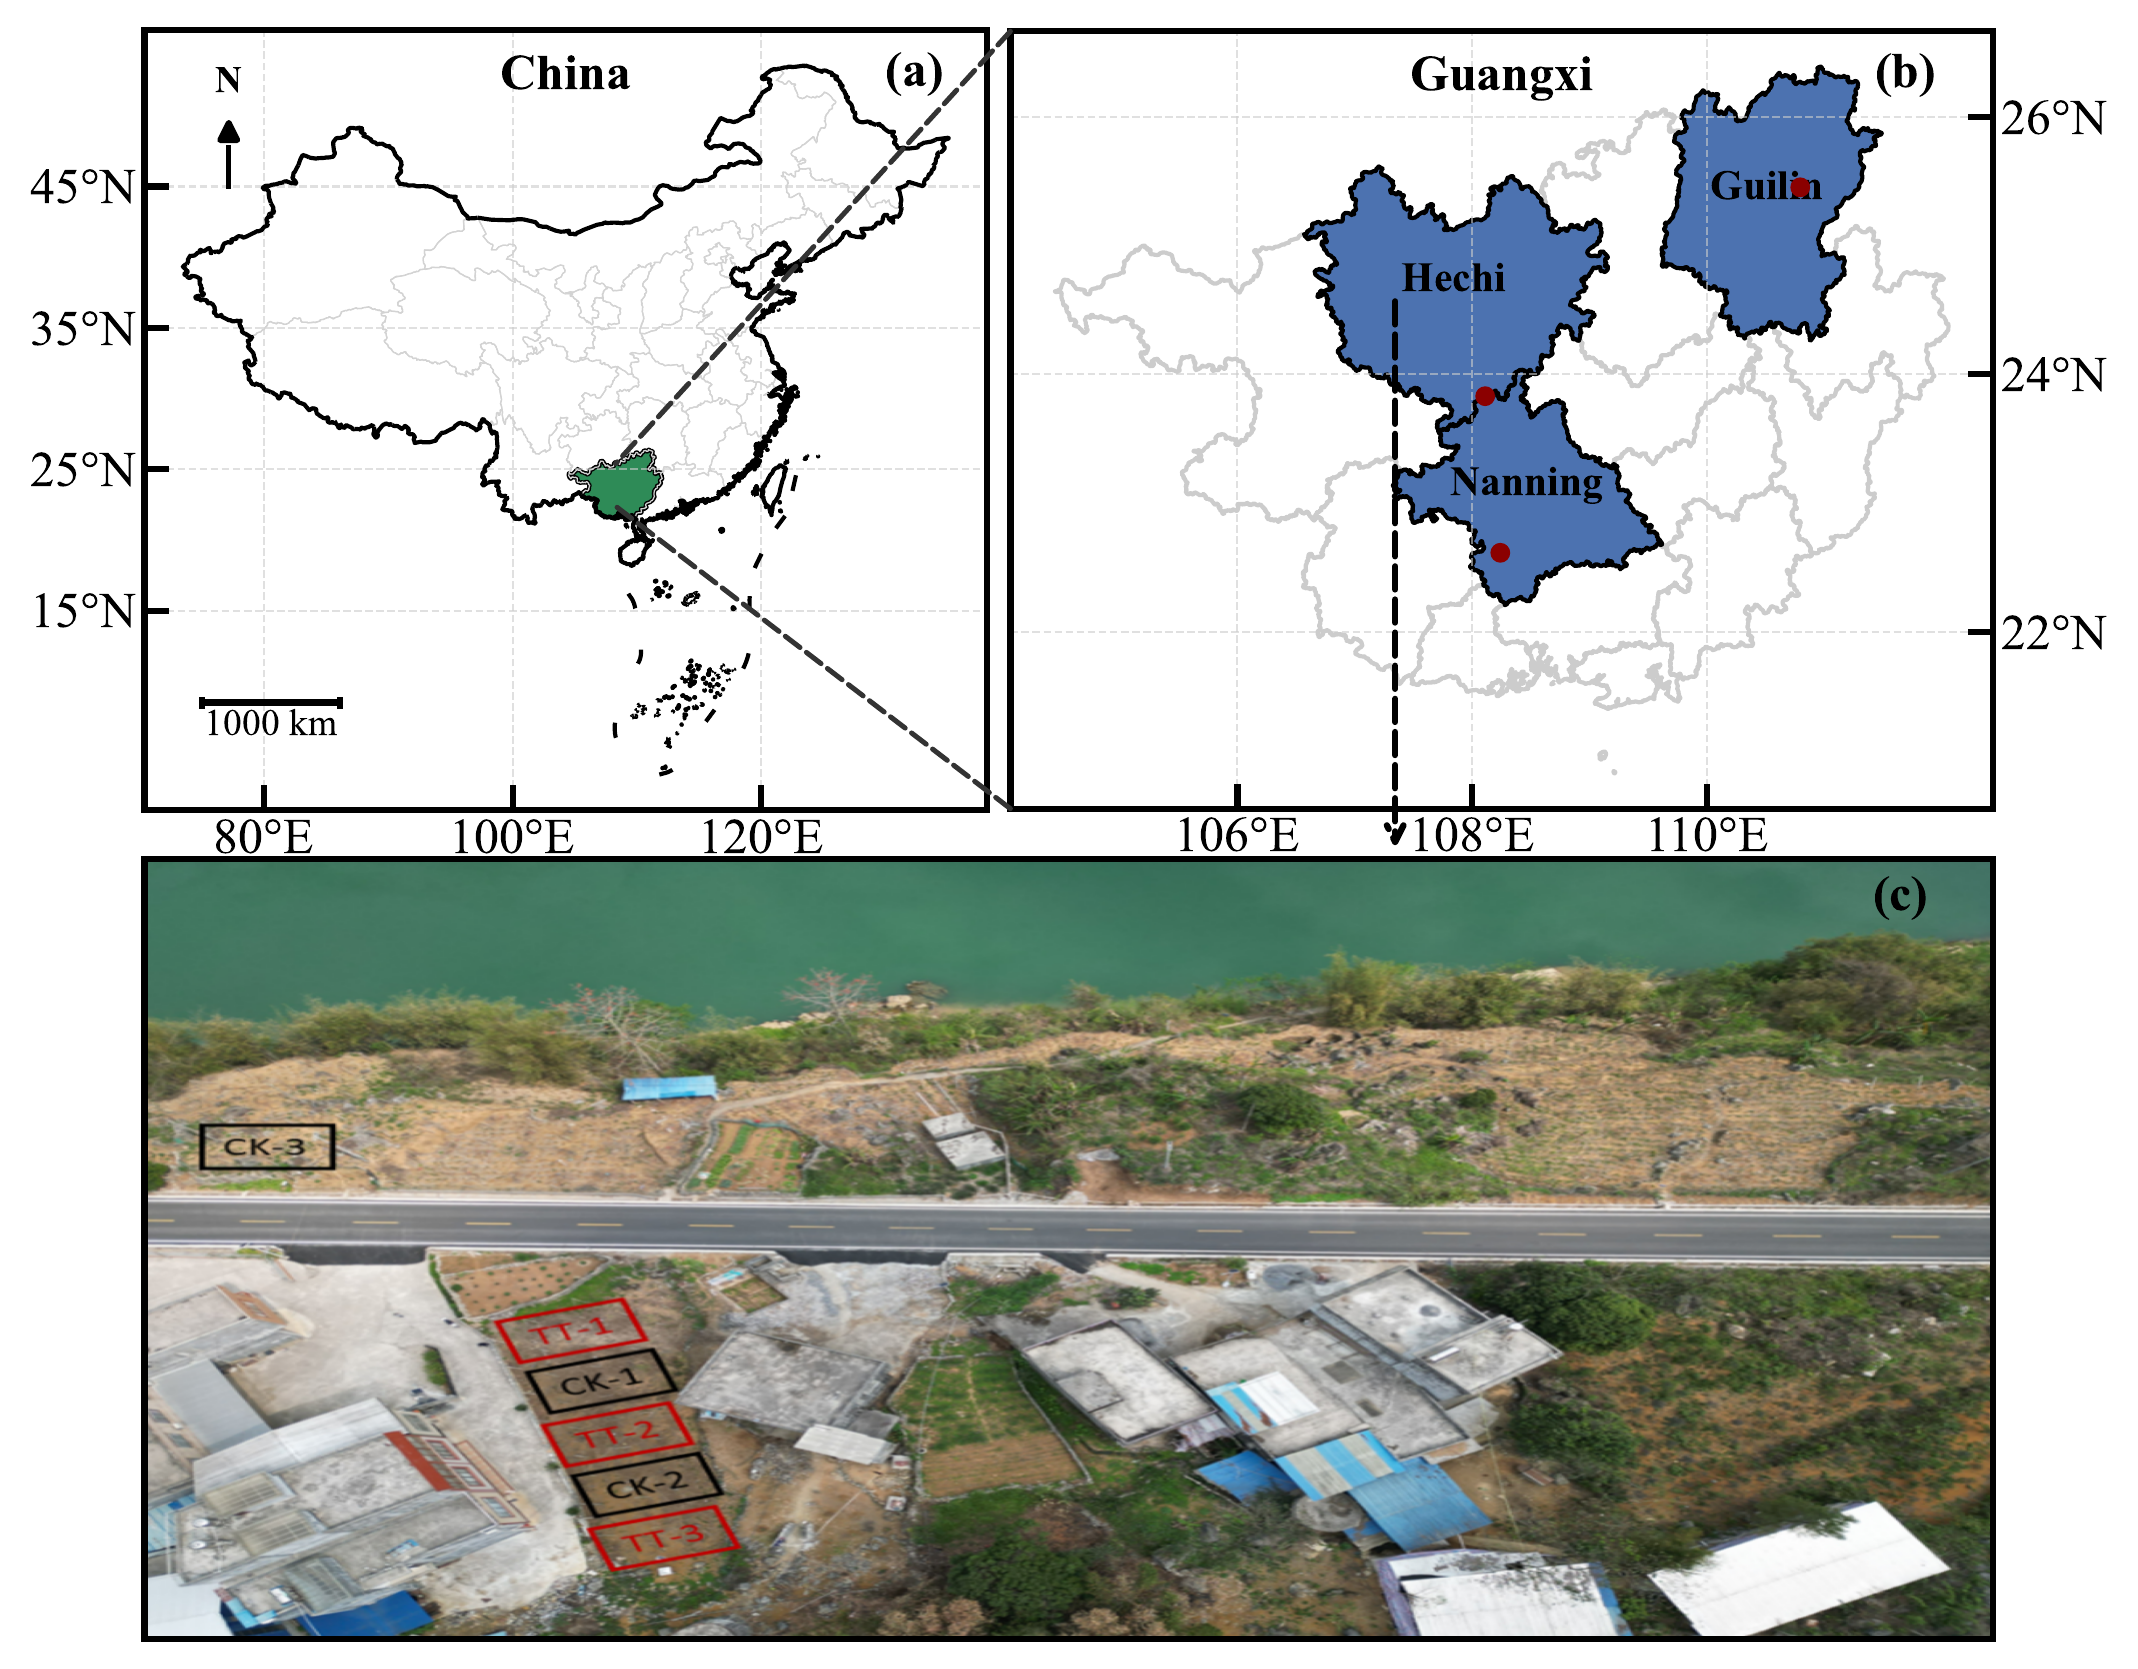
\includegraphics[width=0.95\linewidth]{fig/Figure_02.png}
\caption{Study sites and field layout. (a) Location of Guangxi within
China. (b) Spatial distribution of the three field experiment sites
(Guilin, Hechi, and Nanning) in Guangxi Province; red circles indicate
the locations of the experimental orchards. (c) Plot layout at the
Du'an site in Hechi City, where black rectangles denote the three
untreated control plots (CK).}
\label{_Ref212629919}
\end{figure}

\begin{figure}[H]
\centering
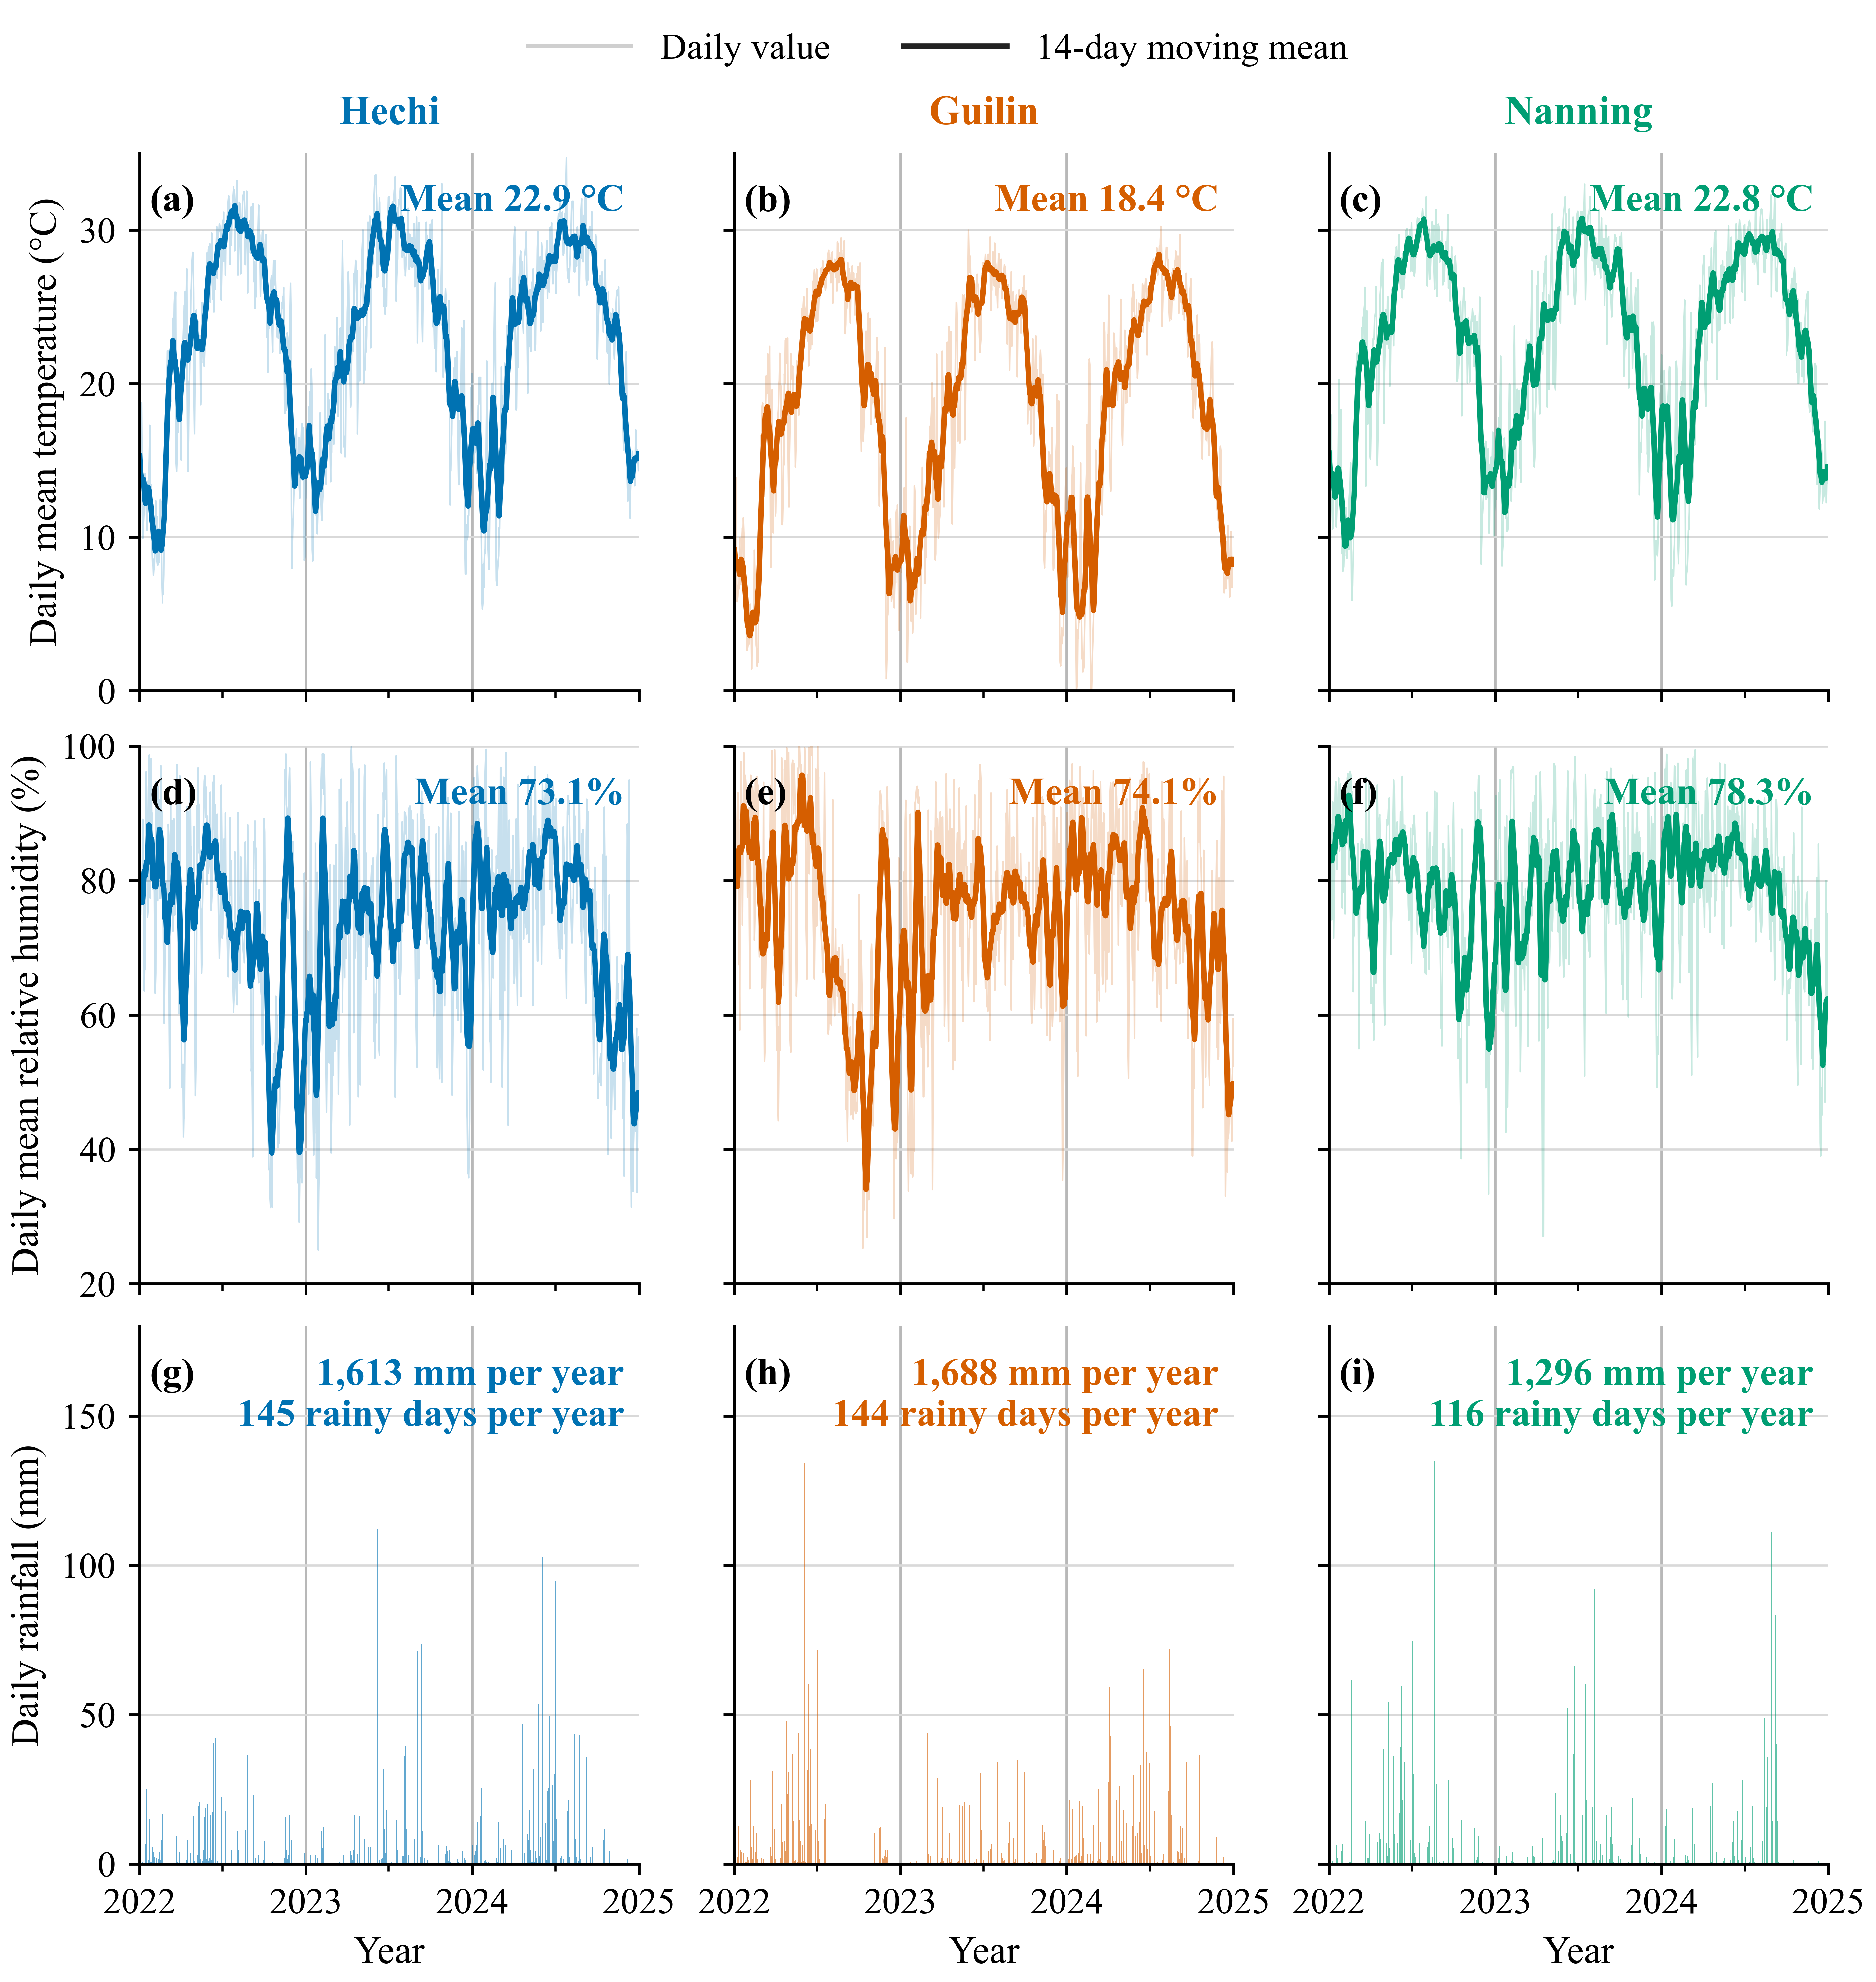
\includegraphics[width=0.95\linewidth]{fig/Figure_03.png}
\caption{Daily mean temperature, daily mean relative humidity, and
daily rainfall recorded at the experimental vineyards in Hechi, Guilin,
and Nanning during 2022--2024. The numerical values shown in each panel
denote the 3-year means of the corresponding variable across all sites,
providing an overview of the background meteorological conditions within
the experimental region.}
\label{_Ref214271335}
\end{figure}

\subsubsection{Disease and phenology data
collection}\label{disease-and-phenology-data-collection}

Grapevine phenological development and downy mildew progression were
monitored throughout the growing season following a standardized field
observation protocol. All assessments were conducted in situ by trained
technicians and recorded using a dedicated WeChat-based mobile data
collection system (``Nong Qing Zhu Shou''), which provided structured
interfaces for extended BBCH coding, lesion annotation, automatic
time-stamping, GPS geolocation, and image capture. Records were uploaded
directly to a cloud database, allowing continuous checks of data
completeness and internal consistency.

Phenological development was recorded according to the extended BBCH
scale for grapevine (Lorenz et al., 1995), from BBCH 00 (dormancy) to
BBCH 99 (harvest). Observation frequency was adjusted according to
developmental stage: from BBCH 00 to BBCH 13 (dormancy to three unfolded
leaves), surveys were conducted weekly; thereafter, as vines entered the
susceptible period for downy mildew and meteorological conditions became
more favourable for infection, inspection frequency increased to once
every two days. In each observation plot, two vines were permanently
tagged as repeated observation units. Leaves along the main shoots were
systematically inspected from lower to upper canopy positions, with both
adaxial and abaxial surfaces inspected for characteristic symptoms.

When suspected lesions were observed, high-resolution images were
captured and centrally reviewed for confirmation. For each vineyard, the
calendar date on which the first oil spot was confirmed in any
observation plot was defined as the timing of first seasonal infection
(\hyperref[_Ref214184122]{Fig 4b}). In addition to first seasonal
infection timing, disease incidence (proportion of symptomatic leaves)
and severity were subsequently assessed on the same tagged vines to
characterize seasonal disease development. For model development and
validation, only confirmed first seasonal infection dates were used,
whereas the full phenological and disease datasets were retained for
complementary analyses of within-season epidemic dynamics.

\begin{figure}[H]
\centering
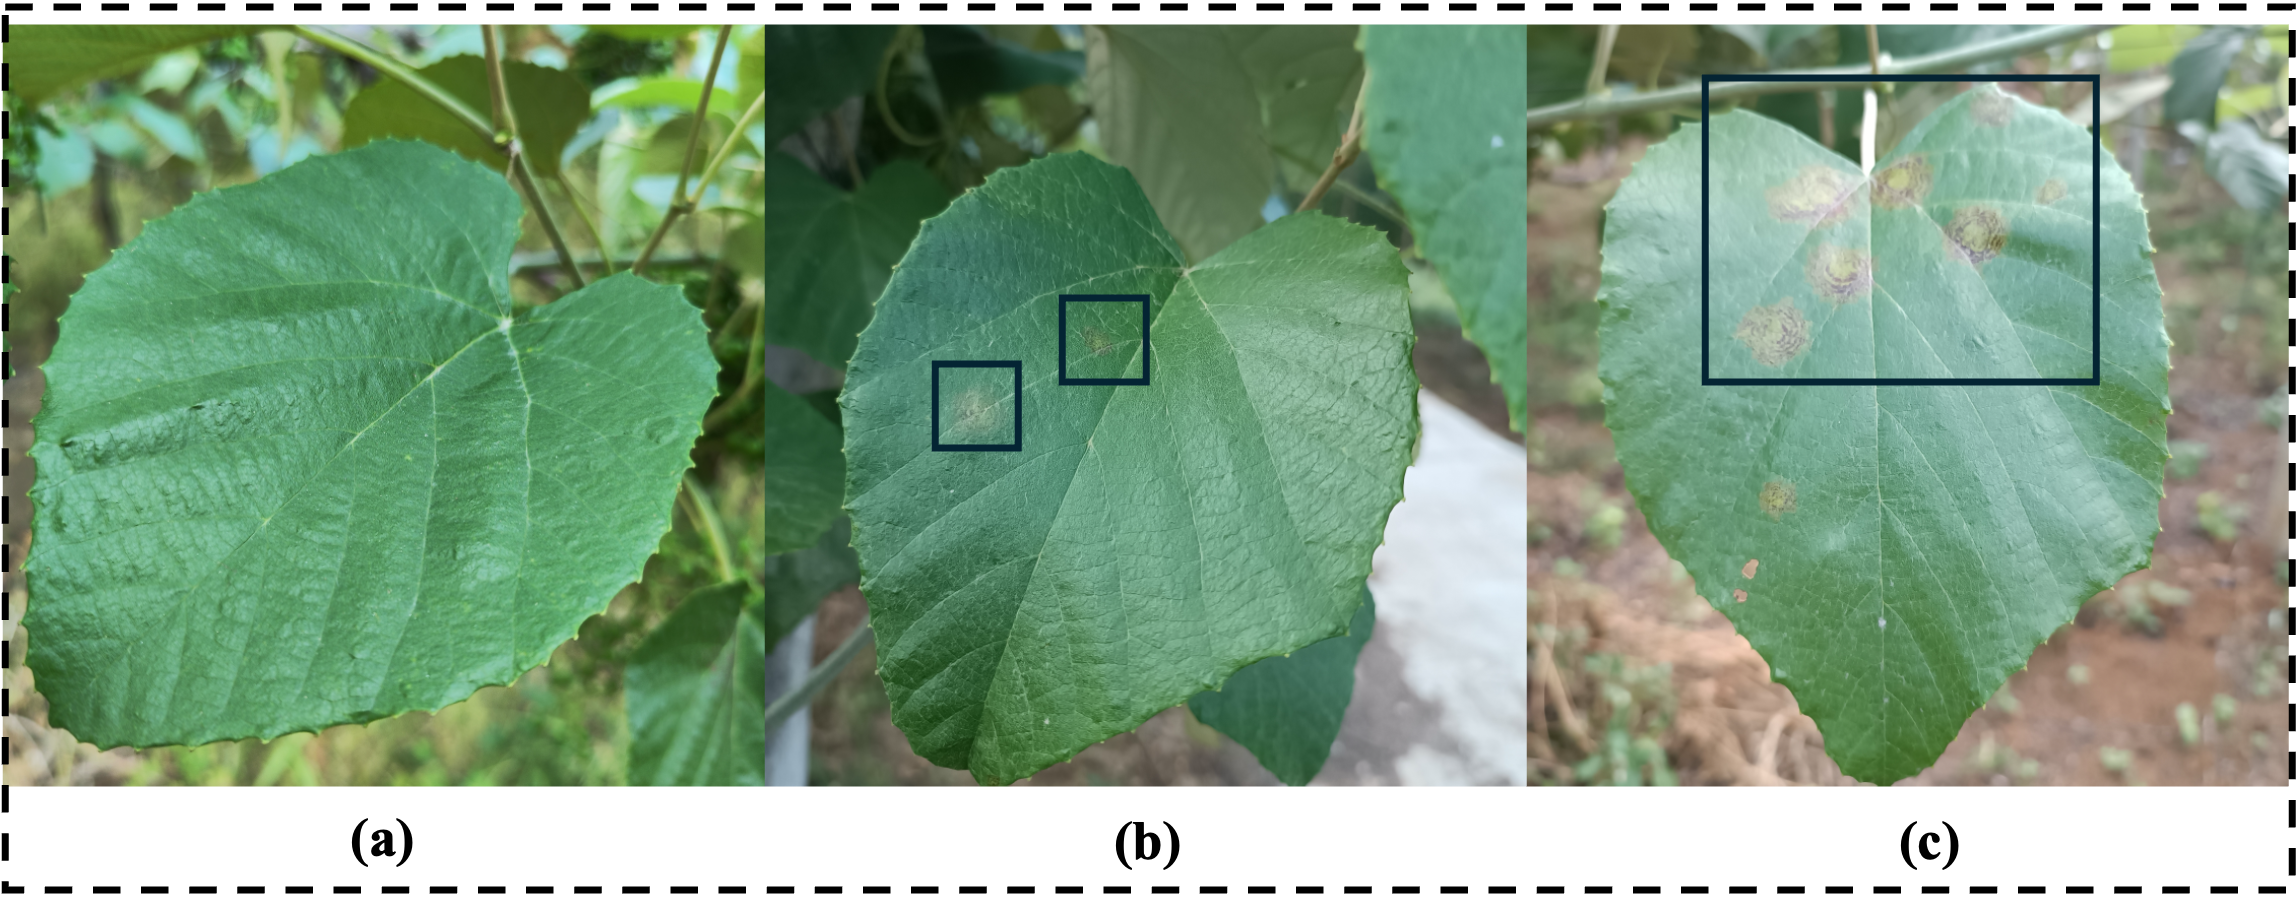
\includegraphics[width=0.90\linewidth]{fig/Figure_04.png}
\caption{Downy mildew lesion emergence and development on Yeniang No. 2
(MPT) leaves in the Du'an experimental vineyard, Hechi. Panels show
severity levels from a single-leaf perspective: (a) healthy; (b) 1\%
(post-incubation visible lesion); (c) 5\%. Photos by team member Qi
Tian (2023).}
\label{_Ref214184122}
\end{figure}

\subsubsection{Airborne sporangia
monitoring}\label{airborne-sporangia-monitoring}

At each vineyard, one passive spore trap (model TPBZ1, Zhejiang Top
Cloud-Agri Technology Co., Ltd., China) was installed adjacent to the
fungicide-free control (CK) plot to monitor the natural airborne
dispersal of \emph{P. viticola} sporangia. Trap placement
avoided potential chemical interference, and the air inlet was
positioned approximately 1.5 m above ground level, corresponding to the
average grapevine canopy height.

Sporangia were collected on glass slides coated with a thin layer of
Vaseline, which were replaced every two days. Samples were sealed and
transported to the laboratory of the Guangxi Academy of Agricultural
Sciences for quantitative analysis. To improve counting accuracy, two
microscopic observation procedures were applied: (i) direct imaging, in
which untreated slides were examined directly under a microscope
(\hyperref[_Ref214187767]{Fig 5b--d}); and (ii) wash imaging, in which
each slide was rinsed with 300 \(\mu\)L of sterile water, and five 30 \(\mu\)L
subsamples were collected from different depths of the rinse solution to
minimize bias associated with particle sedimentation
(\hyperref[_Ref214187767]{Fig 5b--d}). Subsamples were transferred to
concave glass slides for microscopic observation and imaging.

Images obtained from wash imaging were processed using a sporangia
recognition platform developed by our research team
(\url{http://116.10.197.212:9060/spore/\#/}) to support efficient
screening and counting. The platform uses a detection model trained for
\emph{P. viticola} sporangia recognition (Yan et al., 2024). Because
the present study focuses on field-based inoculum monitoring and
agroclimatic disease modelling rather than image-analysis development,
all automatically detected results were independently verified by two
trained laboratory technicians before being used in model calibration and
validation (\hyperref[_Ref214187767]{Fig 5c}).

\begin{figure}[H]
\centering
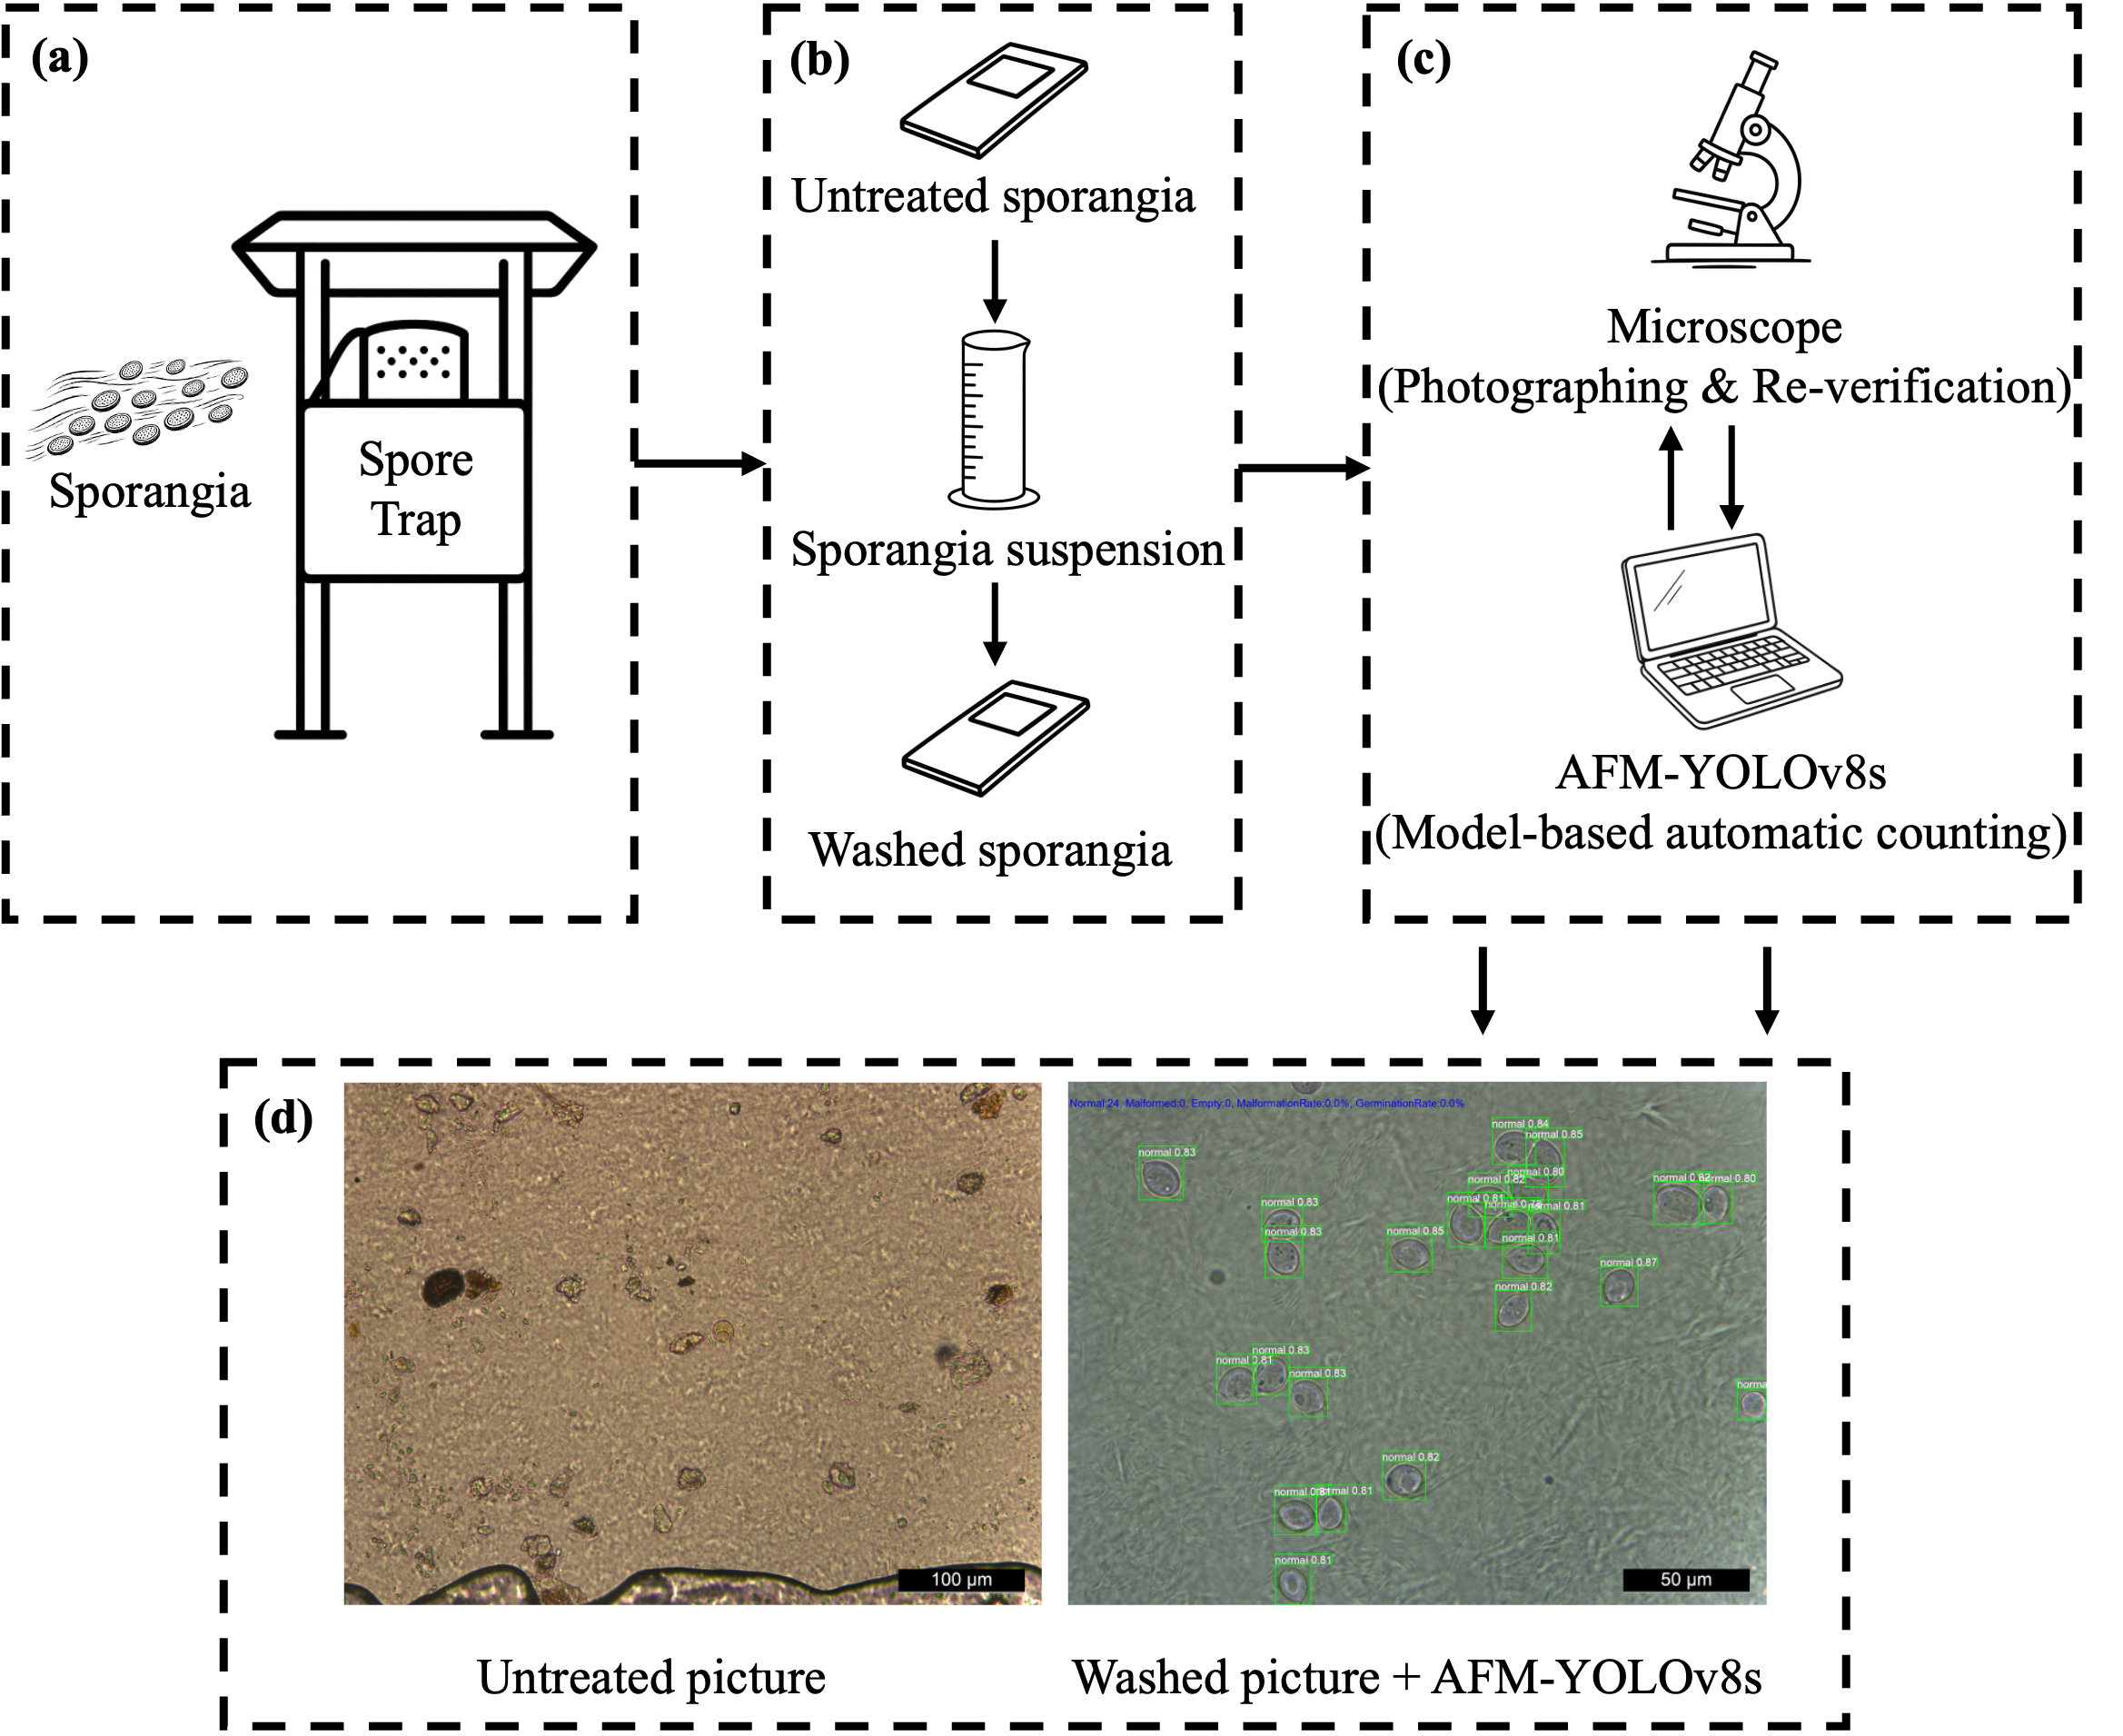
\includegraphics[width=0.95\linewidth]{fig/Figure_05.png}
\caption{Schematic illustration of sporangia collection and processing
in the vineyard experiment. (a) Schematic of dynamic monitoring of
sporangia; (b) schematic of laboratory preprocessing; (c) schematic of
sporangia image and quantity acquisition; (d) representative sporangia
images obtained from the untreated sporangia slide and the washed
sporangia slide.}
\label{_Ref214187767}
\end{figure}

\subsubsection{Meteorological data}\label{meteorological-data}

Meteorological data were retrieved from the Open-Meteo platform
(\href{https://open-meteo.com/}{\ul{https://open-meteo.com/}}), which
provides ERA5 reanalysis products with hourly temporal resolution
(Hersbach et al., 2020). For each experimental orchard, geographic
coordinates were used to extract site-specific time series of air
temperature (T), relative humidity (RH), and precipitation (R). To meet
the requirements of the disease prediction model, additional
variables---including vapor pressure deficit (VPD) and leaf wetness
duration (LWD)---were derived from temperature and humidity data using
the established formulations described by Rossi et al. (2008).

\subsection{Model structure and
refinements}\label{model-structure-and-refinements}

\subsubsection{First Seasonal Infection Model (FSIM): baseline
mechanistic
framework}\label{first-seasonal-infection-model-fsim-baseline-mechanistic-framework}

In this study, the first visible infection event of a new growing
season, primarily driven by asexual sporangia, is defined as the ``First
Seasonal Infection'' event (Fig. S2). Based on
this epidemiological context, a \emph{First Seasonal Infection Model}
(FSIM) was developed to simulate the timing of initial infection events
in subtropical vineyards in Guangxi, China.

Unlike conventional primary infection models that typically initiate
simulations on January 1, the present study used BBCH53 (flowering
stage) of the new growing season as the simulation starting point under
subtropical conditions (Hui et al., 2022). BBCH53 dates were obtained
from field phenological observations and applied as a temporal gating
condition to define the onset of infection simulations.

The FSIM was constructed through structural integration and process
reorganization of the Rossi primary infection model and secondary
infection risk frameworks (Brischetto et al., 2021; Rossi et al., 2008).

Infection-development processes retained from the Rossi model include
zoospore release and survival, infection establishment, incubation, and
symptom expression, which constitute the mechanistic backbone of the
infection chain. The secondary infection risk module was positioned
upstream to describe the production of sporangia, followed by the
infection chain derived from the Rossi model, including zoospore release
and survival, infection establishment, incubation, and symptom
expression. In this restructuring, the probability-accumulation
formulation of the original secondary infection model was reformulated
into a cohort-based representation describing spore production,
accumulation, depletion, and release. Dispersal mechanisms were
distinguished into rainfall-driven and wind-driven pathways. Apart from
process reordering and structural adjustments, the original mathematical
formulations were retained where applicable.

To represent dispersal dynamics, a cohort-based dispersal--deposition
mechanism was introduced (Rossi et al., 2008). The model first updates
the attached sporangia pool \(A_{t}\), which decays during daytime as a
function of vapor pressure deficit (VPD). When \(A_{t}\) falls below a
minimum threshold \(A_{\min}\), no dispersal occurs. A dispersal event
is triggered when hourly rainfall \(R_{t}\) exceeds the rainfall
threshold \(R_{\min}\) or wind speed \(W_{t}\) exceeds the wind
threshold \(W_{\min}\). A single dispersal event is assumed to fully
transfer the attached sporangia pool into the airborne compartment:

\begin{equation}
B_{t_{0}} = A_{t_{0}},\ A_{t_{0}} \rightarrow 0
\tag{1}
\end{equation}

where \(t_{0}\) denotes the dispersal time and \(B_{t_{0}}\) the initial
airborne sporangia amount.

Two dispersal scenarios are distinguished:

Rainfall-driven dispersal: sporangia are assumed to deposit rapidly on
plant surfaces approximately one hour after dispersal:

\begin{equation}
t_{d} = t_{0} + 1\text{~h},\ D = B_{t_{0}}
\tag{2}
\end{equation}

Wind-driven dispersal: sporangia remain airborne and decay exponentially
during daytime:

\begin{equation}
B_{t + 1} = B_{t}\exp( - \lambda_{t})
\tag{3}
\end{equation}

where \(\lambda_{t}\) is a VPD-dependent decay rate. Subsequent
rainfall events exceeding the deposition threshold
\(R_{\min}\) trigger deposition, with deposited inoculum given by:

\begin{equation}
D = B(t_{d}^{-})
\tag{4}
\end{equation}

If the deposited amount falls below the minimum spore threshold, the
cohort is considered inactive and does not contribute to subsequent
infection processes.

Field monitoring indicated that airborne pathogen structures captured
prior to the appearance of visible lesions were predominantly sporangia
(\hyperref[_Ref214187767]{Fig 5d}), providing observational support for
the sporulation, dispersal, and deposition modules included in the FSIM.

\subsubsection{\texorpdfstring{Spore-constrained refinement of the
\emph{First Seasonal Infection Model}
(FSIM-S)}{Spore-constrained refinement of the First Seasonal Infection Model (FSIM-S)}}\label{spore-constrained-refinement-of-the-first-seasonal-infection-model-fsim-s}

An extended model (FSIM-S) was developed while maintaining the
mechanistic process chain of FSIM. The suffix ``-S'' denotes the
incorporation of airborne sporangia observations. A daily sporangia
pressure field \(S(d)\) was constructed from field monitoring data. After
temporal interpolation, normalization, and smoothing, the resulting
signal represented relative inoculum pressure conditions. Hourly spore
pressure was defined as a three-day rolling average:

\begin{equation}
P_{t} = \frac{1}{3}\sum_{k = 0}^{2}\mspace{2mu}\mspace{2mu} S(d_{t} - k)
\tag{5}
\end{equation}

In the baseline FSIM, infection occurrence was determined by:

\begin{equation}
WD_{t} \cdot TWD_{t} \geq IC
\tag{6}
\end{equation}

where \(IC\) denotes the infection threshold parameter. In FSIM-S, this
fixed threshold was replaced by a pressure-adjusted effective threshold
\(IC_{t}^{*}\):

\begin{equation}
IC_{t}^{*} = \left\{ \begin{matrix}
IC \cdot \exp( - \alpha_{pos}P_{t}), & P_{t} \geq 0, \\
IC \cdot \exp(\alpha_{neg}( - P_{t})), & P_{t} < 0
\end{matrix} \right.
\tag{7}
\end{equation}

and infection was considered to occur when:

\begin{equation}
WD_{t} \cdot TWD_{t} \geq IC_{t}^{*}
\tag{8}
\end{equation}

where \(\alpha_{pos}\) and \(\alpha_{neg}\) are calibration parameters
controlling threshold adjustments under high and low inoculum pressure,
respectively. Apart from this infection-threshold adjustment, all
meteorological drivers and physiological process formulations remained
identical to those in FSIM. The conceptual structure of the baseline and
spore-constrained models is summarized in
\hyperref[_Ref_model_concept]{Fig 6}.

\begin{figure}[H]
\centering
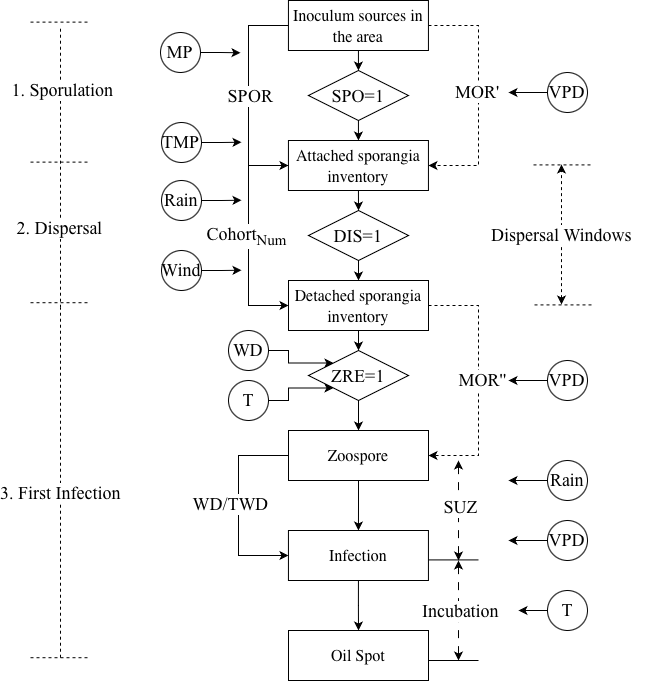
\includegraphics[width=0.90\linewidth]{fig/Figure_06.png}
\caption{Conceptual diagram of the model. The figure illustrates the
mechanistic framework of first seasonal infection by \emph{Plasmopara
viticola} in subtropical Guangxi (FSIM). Red text indicates the
incorporation of an observed spore-pressure field during the infection
stage, representing the refined model denoted as FSIM-S.}
\label{_Ref_model_concept}
\end{figure}

\subsection{Parameterization and sensitivity
analysis}\label{parameterization-and-sensitivity-analysis}

To identify key parameters and compare parameter response patterns
before and after incorporation of spore information, global sensitivity
analyses were conducted for both the baseline \emph{First Seasonal
Infection Model} (FSIM) and the spore-constrained enhanced model
(FSIM-S). Considering the relatively high dimensionality of model
parameters and computational cost, a Morris global sensitivity analysis
framework (Morris, 1991; Iooss and Lemaître, 2015) adopted to evaluate
the relative influence of parameters on model outputs and to detect
potential nonlinear and interaction effects. Parameter sampling and
sensitivity index estimation were implemented using the SALib toolkit.
The number of sampling levels was set to six, and 256--512 trajectories
were generated to balance computational efficiency and stability of
sensitivity estimates. Model performance was evaluated based on the
difference in day-of-year (DOY) between observed first lesion appearance
and the simulated oil-spot occurrence window, using mean absolute error
(MAE) as the primary metric. When no effective infection event was
simulated, a fixed penalty error (120 d) was applied to maintain
statistical consistency. The penalty value was selected to exceed the
biologically plausible infection window within a single growing season.

Let \(x = (x_{1},\ldots,x_{k})\) denote the parameter vector and
\(f(x)\) the model output. Following the Morris method, the elementary
effect of the \(i\)-th parameter at sampling point \(\mathbf{x}\) is
defined as:

\begin{equation}
EE_{i}(x) = \frac{f(x_{1},\ldots,x_{i} + \Delta,\ldots,x_{k}) - f(x)}{\Delta}
\tag{9}
\end{equation}

Here, \(\Delta\) denotes the step size in the normalized parameter
space, determined by the predefined number of sampling levels. Based on
\(N\) elementary effects, three sensitivity statistics were calculated:

\begin{equation}
\mu_{i} = \frac{1}{N}\sum_{j = 1}^{N}\mspace{2mu}\mspace{2mu} EE_{i,j},\ {\ \mu}_{i}^{*} = \frac{1}{N}\sum_{j = 1}^{N}\mspace{2mu}\mspace{2mu}|EE_{i,j}|
\tag{10}
\end{equation}

\begin{equation}
\sigma_{i} = \sqrt{\frac{1}{N - 1}\sum_{j = 1}^{N}\mspace{2mu}\mspace{2mu}{(EE_{i,j} - \mu_{i})}^{2}}
\tag{11}
\end{equation}

Among these, \(\mu_{i}^{*}\) represents the overall influence magnitude
of a parameter and serves as the primary indicator for identifying key
parameters; \(\mu_{i}\) reflects the directional effect (advancing or
delaying infection timing); and \(\sigma_{i}\) captures nonlinear effects
and parameter interactions. Parameters were ranked according to
\(\mu_{i}^{*}\) to support parameter screening and subsequent model
calibration.

Regarding parameterization, the FSIM parameter set
(\hyperref[_Ref226058574]{Table 2}) largely inherits biologically
interpretable parameters from established grapevine downy mildew
mechanistic models, with selected parameter ranges adjusted based on
subtropical vineyard observations. The FSIM-S model further introduces
spore-pressure adjustment parameters (\hyperref[_Ref226058574]{Table 2})
to account for dynamic modulation of infection triggering thresholds by
airborne inoculum pressure. Comparing sensitivity structures under a
unified analytical framework enables quantitative assessment of how
incorporation of spore information modifies parameter control patterns
and supports subsequent model refinement and calibration.

\protect\phantomsection\label{_Ref226058574}{}
\begin{center}
\textbf{Table 2} Model parameters under the FSIM and FSIM-S frameworks.
FSIM denotes the baseline model, whereas FSIM-S represents the extended
version incorporating regulation by an observed spore-pressure field.
\end{center}

{\def\LTcaptype{none} % do not increment counter
\begin{longtable}[]{@{}
  >{\raggedright\arraybackslash}p{(\linewidth - 10\tabcolsep) * \real{0.3342}}
  >{\raggedright\arraybackslash}p{(\linewidth - 10\tabcolsep) * \real{0.1404}}
  >{\raggedright\arraybackslash}p{(\linewidth - 10\tabcolsep) * \real{0.0964}}
  >{\raggedright\arraybackslash}p{(\linewidth - 10\tabcolsep) * \real{0.0964}}
  >{\raggedright\arraybackslash}p{(\linewidth - 10\tabcolsep) * \real{0.0743}}
  >{\raggedright\arraybackslash}p{(\linewidth - 10\tabcolsep) * \real{0.2584}}@{}}
\toprule\noalign{}
\begin{minipage}[b]{\linewidth}\raggedright
Parameter
\end{minipage} & \begin{minipage}[b]{\linewidth}\raggedright
Abbreviation
\end{minipage} & \begin{minipage}[b]{\linewidth}\raggedright
FSIM
\end{minipage} & \begin{minipage}[b]{\linewidth}\raggedright
FSIM-S
\end{minipage} & \begin{minipage}[b]{\linewidth}\raggedright
Unit
\end{minipage} & \begin{minipage}[b]{\linewidth}\raggedright
Description
\end{minipage} \\
\midrule\noalign{}
\endhead
\bottomrule\noalign{}
\endlastfoot
Mp\_tmp\_\_rh\_wet\_night & MTWN & 87.5894 & 83.6223 & \% & Night-time
relative humidity threshold used to define wet-night conditions for
sporulation initiation. \\
Sporulation\_\_MP\_min & SMMI & 4.3106 & 5.1741 & hours & VPD threshold
representing Minimum cumulative wet-night hours required to trigger
sporulation. \\
Sporulation\_\_Tmin & STMI & 13.9426 & 11.8061 & °C & Lower temperature
limit for sporulation response. \\
Sporulation\_\_Topt & STOP & 25.4161 & 19.3980 & °C & Optimum
temperature for sporulation intensity. \\
Sporulation\_\_Tmax & STMX & 35.2136 & 35.0492 & °C & Upper temperature
limit for sporulation response. \\
Dispersal\_\_rain\_min & DIRM & 12.4525 & 12.3417 & mm & Rainfall
threshold triggering rain-driven sporangial dispersal. \\
Dispersal\_\_wind\_min & DIWM & 6.4975 & 6.2638 & m/s & Wind-speed
threshold triggering wind-driven sporangial dispersal. \\
Deposition\_\_rain\_min & DERM & 5.1413 & 6.0721 & mm & Rainfall
threshold controlling deposition/washout of airborne propagules. \\
Zoospore\_alive\_\_rain & ZARA & 4.0835 & 5.3267 & mm & Rainfall
condition threshold used in zoospore survival gating. \\
Zoospore\_alive\_\_vpd & ZVPD & 1.9396 & 1.9674 & kPa & Vapor pressure
deficit threshold used in zoospore survival gating. \\
Infection\_\_infection\_condition & IC & 25.4409 & 81.4294 & / &
Infection requirement threshold. \\
Incubation\_\_spl\_spores & ISED & 1.1063 & 0.9361 & / & Cumulative
incubation progress threshold for visible oil-spot onset. \\
Thresholds\_\_min\_spores & TMSO & 0.0431 & 0.1016 & / & Minimum viable
spore amount retained for process continuity. \\
Spore\_\_alpha\_pos & SAP & / & 1.2849 & / & Positive spore-pressure
coefficient; decreases effective infection threshold under favourable
spore pressure. \\
Spore\_\_alpha\_neg & SAN & / & 0.6306 & / & Negative spore-pressure
coefficient; increases effective infection threshold under suppressive
spore pressure. \\
\end{longtable}
}

\subsection{Model calibration and
evaluation}\label{model-calibration-and-evaluation}

To assess the temporal predictive capability and applicability of the
\emph{First Seasonal Infection Model} (FSIM) and its spore-constrained
extension (FSIM-S) under humid subtropical vineyard conditions,
parameter calibration and model evaluation were conducted within a
unified methodological framework. Both models employed identical
calibration strategies and evaluation metrics, while FSIM-S additionally
incorporated a spore-pressure field derived from airborne sporangia
observations together with associated adjustment parameters, allowing
quantitative assessment of the effect of incorporating inoculum
information into the infection simulation process.

\subsubsection{Calibration strategy}\label{calibration-strategy}

Model parameters were optimized using Bayesian optimization based on the
Tree-structured Parzen Estimator (TPE) approach (Bergstra et al., 2011),
which enables efficient exploration of high-dimensional parameter spaces
through probabilistic modelling. The optimization objective was defined
as minimization of the mean absolute error (MAE) in predicted
first-infection timing. Given the relatively large parameter space and
the potential multimodality of the objective function, extensive
parameter exploration was performed (approximately \(2 \times 10^{4}\)
trials for the baseline model and \(3 \times 10^{4}\) trials for the
spore-constrained model).

To enhance robustness of parameter selection, approximately the top 5\%
of high-performing candidate parameter sets identified during
optimization were retained for subsequent comparative evaluation. This
strategy reduces the risk of overfitting and avoids overlooking
near-optimal solutions.

Compared with the baseline FSIM, the FSIM-S model maintains the same
mechanistic infection framework while incorporating a daily airborne
spore-pressure field derived from field observations. Additional
parameters were introduced to dynamically adjust infection-triggering
thresholds according to inoculum pressure. Apart from these
spore-related parameters, both models used identical meteorological
drivers, biological process formulations, and calibration procedures to
ensure comparability of predictive performance. Parameter ranges were
constrained based on biologically plausible values derived from previous
mechanistic studies and field observations to maintain ecological
realism.

\subsubsection{Performance metrics}\label{performance-metrics}

Model performance was primarily evaluated using temporal prediction
error metrics. Mean absolute error (MAE) and root mean square error
(RMSE) were calculated to quantify overall prediction accuracy and
sensitivity to large deviations:

\begin{equation}
MAE = \frac{1}{n}\sum_{i = 1}^{n}\mspace{2mu}\mspace{2mu}\left| y_{i} - {\widehat{y}}_{i} \right|
\tag{12}
\end{equation}

\begin{equation}
RMSE = \sqrt{\frac{1}{n}\sum_{i = 1}^{n}\mspace{2mu}\mspace{2mu}{\left( y_{i} - {\widehat{y}}_{i} \right)}^{2}}
\tag{13}
\end{equation}

where \(y_{i}\) and \({\widehat{y}}_{i}\) denote observed and simulated
first-infection dates expressed as day-of-year (DOY), respectively, and
\(n\) is the number of observations.

When no effective infection event was simulated or numerical anomalies
occurred, a fixed penalty error of 120 days was assigned. This value
substantially exceeds the plausible temporal range for first seasonal
infection within a single growing season and was applied to ensure
consistent penalization of missed infection events during statistical
comparison.

\subsubsection{Cross-validation and robustness
assessment}\label{cross-validation-and-robustness-assessment}

To avoid bias associated with fixed training--validation splits, a
three-fold cross-validation scheme was applied in which site-year
datasets were randomly partitioned into three subsets, each serving once
as validation data while the remaining subsets were used for
calibration.

To ensure reproducibility of parameter optimization, a fixed random seed
(seed = 42) was used for data partitioning and optimization
initialization. Final model performance was summarized using
fold-averaged MAE and RMSE values, with corresponding standard
deviations reported to reflect predictive stability and cross-site
generalizability.

\subsubsection{Selection of global parameter
configuration}\label{selection-of-global-parameter-configuration}

To obtain a single deterministic model configuration for site--year
simulations, the fold-specific best parameter sets (those achieving the
lowest validation MAE within each fold) were evaluated on the full
dataset. The configuration yielding the lowest overall MAE was selected
as the final global parameter set. Direct averaging of parameters across
folds was avoided, as it led to substantial error inflation due to the
non-convex nature of the objective function and the presence of multiple
near-optimal parameter regions.

\subsection{Regional simulation and disease-management scenario
analysis}\label{regional-simulation-and-disease-management-scenario-analysis}

To evaluate the applicability of the FSIM-S model at the regional scale
and its potential value for risk-based disease management, regional
simulations were conducted across Guangxi Province for the period
2000--2024. Given the limited spatial coverage of field observations and
the lack of a spatially explicit vineyard census layer, the regional
analysis was framed as a scenario-based assessment rather than as a
complete mapping of actual vineyard distribution. Three cultivar
scenarios were constructed to ensure comparability across the region,
assuming that vineyards were uniformly planted with Wink, Yeniang No. 2,
or Kyoho cultivars, respectively. The model was driven by the hourly
meteorological dataset described previously (\hyperref[_Ref214271335]{Fig
3}).

Considering that growers in the region commonly adopt similar preventive
spraying schedules through peer-to-peer technical exchange, chemical
disease management was represented using a schedule
derived from the 2022 Du'an (Hechi) experimental vineyard
(\hyperref[_Ref214272651]{Fig 7}) (Chavas and Nauges, 2020; Huffman,
2020; Norton and Alwang, 2020). The potential to avoid early preventive
treatments was evaluated relative to this baseline schedule, whereby any
preventive fungicide application conducted more than seven days before the simulated
first-infection onset was classified as potentially avoidable. The
seven-day buffer was used to remain consistent with the protection
window commonly expected for vineyard fungicide applications and to
avoid classifying near-risk sprays as redundant. Based on this
criterion, the multi-year average number of potentially avoidable early
applications and the corresponding reduction proportion were calculated.

\begin{figure}[H]
\centering
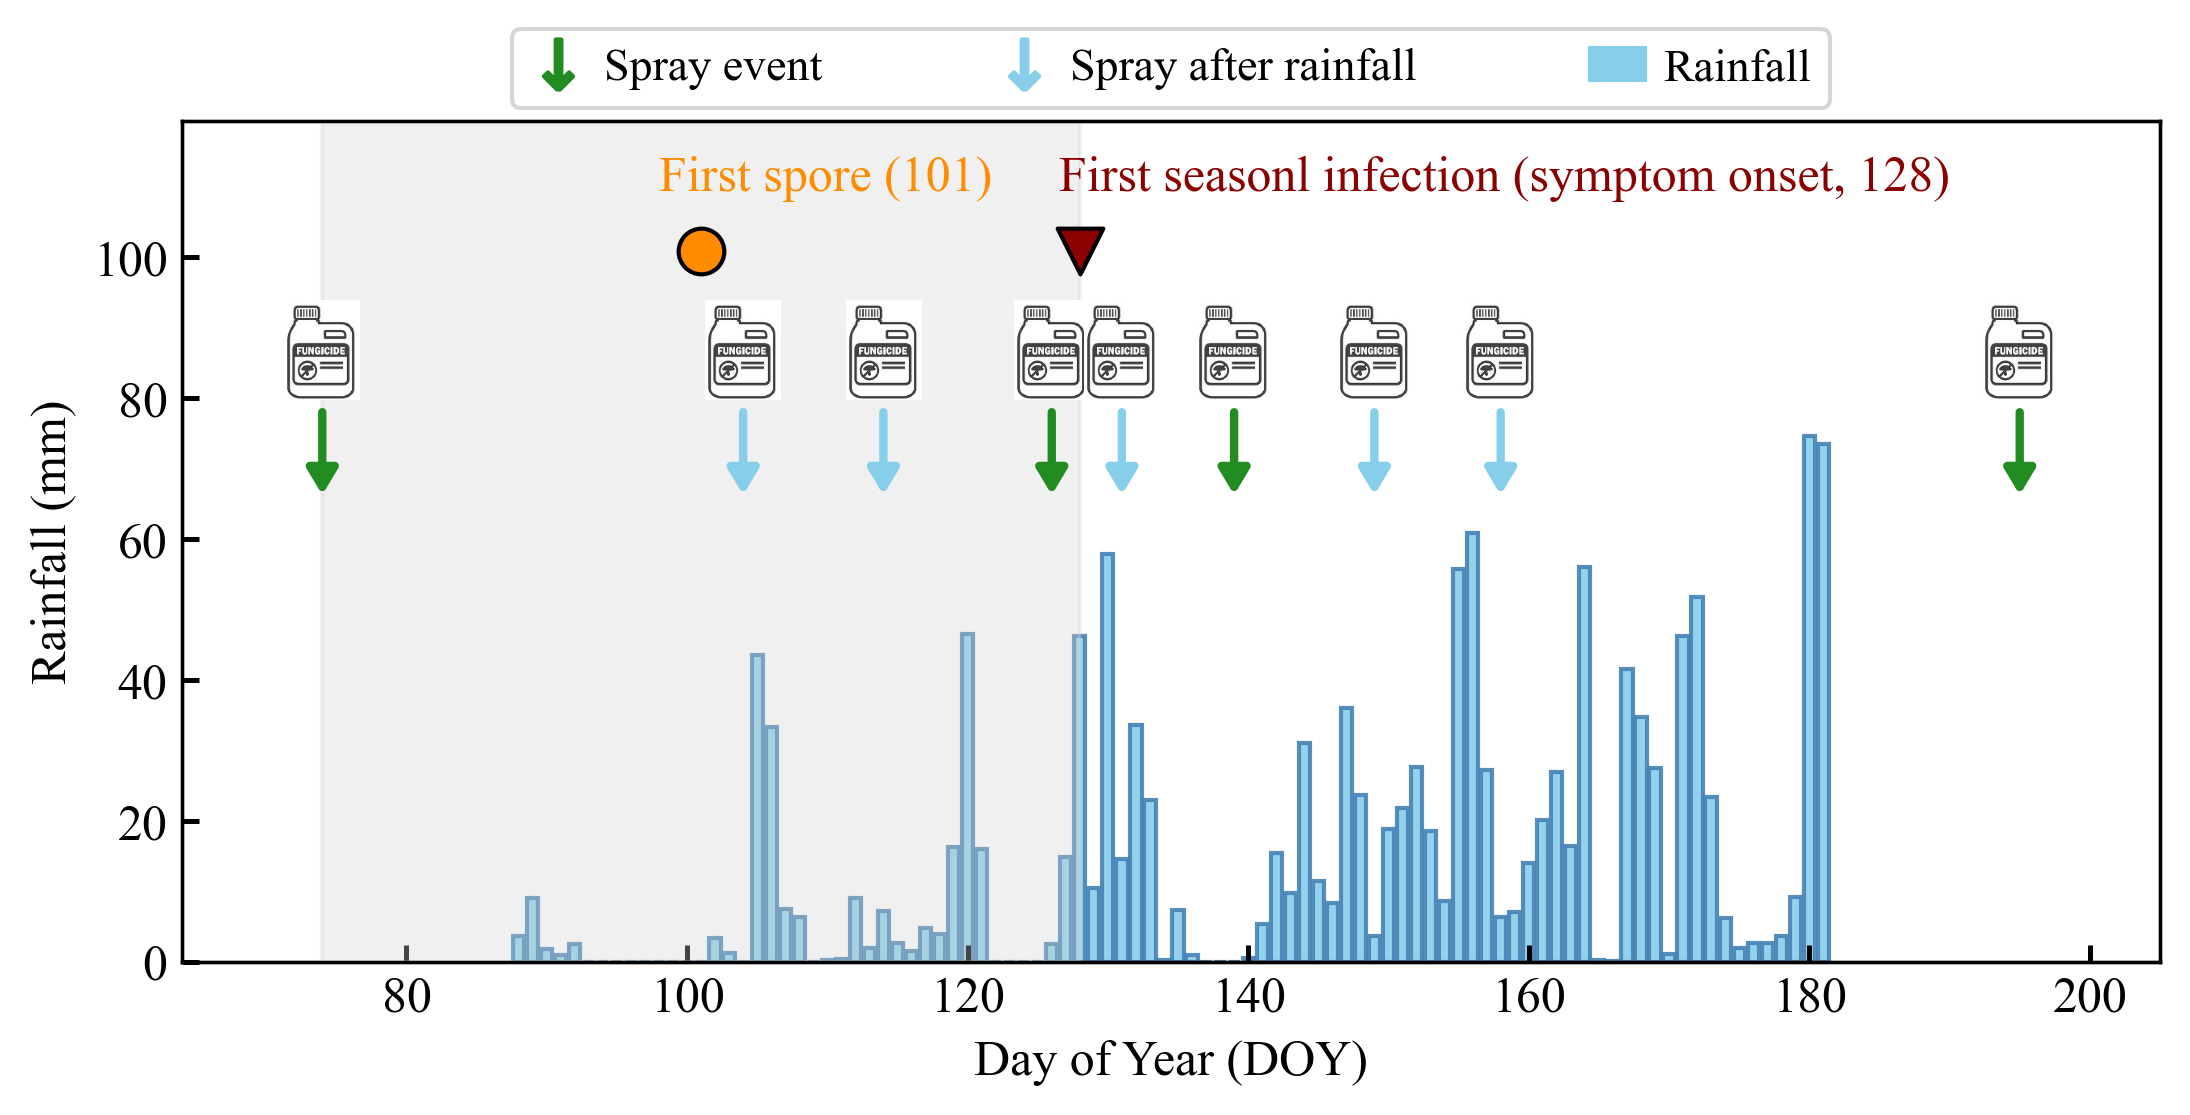
\includegraphics[width=0.95\linewidth]{fig/Figure_07.png}
\caption{Illustration of the empirically executed fungicide application
pattern, documented by field investigators immediately after each
grower-implemented spray event in the experimental vineyard in Du'an,
Hechi City, during the 2022 growing season. The management practice was
characterized by preventive fungicide applications conducted after
rainfall events and prior to the onset of first seasonal infection. The
shaded region indicates the period of such pre-infection,
rainfall-triggered preventive sprays.}
\label{_Ref214272651}
\end{figure}

\subsubsection{Reconstruction of flowering dates
(BBCH53)}\label{reconstruction-of-flowering-dates-bbch53}

Because continuous observations of the BBCH53 phenological stage
(flowering) were unavailable for most years during 2000--2024, while the
FSIM-S disease model requires this stage as a phenological gate for
infection activation, a meteorology-driven BBCH53 reconstruction module
was developed and calibrated to provide consistent phenological inputs
for regional simulations (Hui et al., 2022).

Phenological development was represented using accumulated thermal time
derived from hourly air temperature. Effective growing degree days (GDD)
for each hour \(h\) were calculated as:

\begin{equation}
GDD_{h} = \frac{\max(T_{h} - T_{base},0)}{24}
\tag{14}
\end{equation}

where \(T_{h}\) denotes hourly air temperature and \(T_{base}\) is the
base temperature. Accumulated thermal time from the starting date
\(t_{0}\ \)(defined by \emph{start\_doy}) was then computed as:

\begin{equation}
AGDD(t) = \sum_{h = t_{0}}^{t}\mspace{2mu}\mspace{2mu} GDD_{h}
\tag{15}
\end{equation}

The BBCH53 date was defined as the first day satisfying both a
cumulative thermal threshold and a short-term heat constraint:

\begin{equation}
AGDD(t) \geq \theta_{AGDD},\ RGDD_{7d}(t) \geq \theta_{RGDD}
\tag{16}
\end{equation}

where \(RGDD_{7d}(t)\) represents the 7-day running sum of daily GDD,
introduced to reduce premature triggering caused by short-term
temperature anomalies.

To account for cultivar differences, thermal thresholds and starting
dates were cultivar-adjusted. The effective thermal threshold was
expressed as:

\begin{equation}
\theta_{eff} = \theta_{AGDD}(1 + \delta_{v} + k_{MPT}z_{y})
\tag{17}
\end{equation}

where \(\delta_{v}\) denotes cultivar-specific threshold offsets (Wink,
Yeniang No. 2, and Kyoho), and \(k_{MPT}z_{y}\) represents an additional
year-type adjustment derived from winter temperature conditions. The
effective starting date was adjusted as:

\begin{equation}
start\_ doy_{eff} = start\_ doy + s_{v}
\tag{18}
\end{equation}

where \(s_{v}\) is the cultivar-specific offset.

Parameter calibration followed a Bayesian optimization framework
combined with cross-validation to improve robustness of parameter
selection. Calibration was conducted in two stages: first optimizing
general thermal parameters (e.g., base temperature, thermal thresholds,
and starting date), and subsequently estimating cultivar adjustment
parameters based on the best-performing candidates. Given the limited
availability of phenological observations, calibration emphasized
obtaining stable and reusable phenological estimates for disease-model
input rather than achieving maximal phenological prediction accuracy.

The final parameter set was used to reconstruct gridded BBCH53 dates
across Guangxi for 2000--2024, and these reconstructed phenological
dates were subsequently used as standardized inputs for regional FSIM-S
disease simulations.

\subsubsection{Reconstruction of spore pressure
fields}\label{reconstruction-of-spore-pressure-fields}

Because continuous airborne spore observations were unavailable for the
historical period (2000--2024), while the FSIM-S model requires inoculum
pressure information to regulate infection triggering, a
meteorology-driven spore-pressure reconstruction module was developed.
Field spore monitoring data collected during 2022--2024 were used for
parameter calibration, after which spatially explicit spore pressure
time series were reconstructed to drive historical simulations.

The module follows a ``potential inoculum reservoir--pressure index''
dynamic framework, in which meteorological effects on spore production
and loss are represented as source and loss terms:

\begin{equation}
A_{t} = \max\left( 0,\rho A_{t - 1} + Source_{t} - Loss_{t} \right)
\tag{19}
\end{equation}

where \(A_{t}\) denotes the latent inoculum state. After logarithmic
normalization and smoothing, the resulting daily spore pressure index
\(S_{t}\) was used as an input variable for infection triggering in
FSIM-S.

To ensure consistency with the disease process model, meteorological
drivers used in pressure reconstruction share the same physical
interpretation as those controlling infection processes in FSIM-S.
However, the pressure module employs a simplified inoculum reservoir
dynamic that is independently calibrated, enabling robust forcing input
under conditions lacking long-term spore observations. Calibration was
performed using Bayesian optimization with cross-validation, and the
resulting parameters were applied to reconstruct gridded spore pressure
fields for 2000--2024, which were subsequently coupled to FSIM-S through
infection-threshold adjustment mechanisms.

\section{Results}\label{results}

\subsection{Field observations of disease onset and spore
dynamics}\label{field-observations-of-disease-onset-and-spore-dynamics}

Among the six datasets collected from Guilin, Hechi, and Nanning between
2022 and 2024, the first detection of airborne \emph{P. viticola} sporangia
occurred between March 30 and April 20, while first seasonal infection
symptoms were observed between April 20 and May 30
(\hyperref[_Ref212492136]{Fig 8}). An exception was noted in the Nanning
vineyard in 2023, where symptom onset was delayed until June. In both
Hechi and Nanning, symptom appearance in 2023 was later than in 2022 and
2024. The interval between initial sporangia detection and symptom onset
varied substantially across sites and years, ranging from 9 days in
Nanning (2024) to 72 days at the same site in 2023, indicating marked
interannual variability in epidemic development.

\begin{figure}[H]
\centering
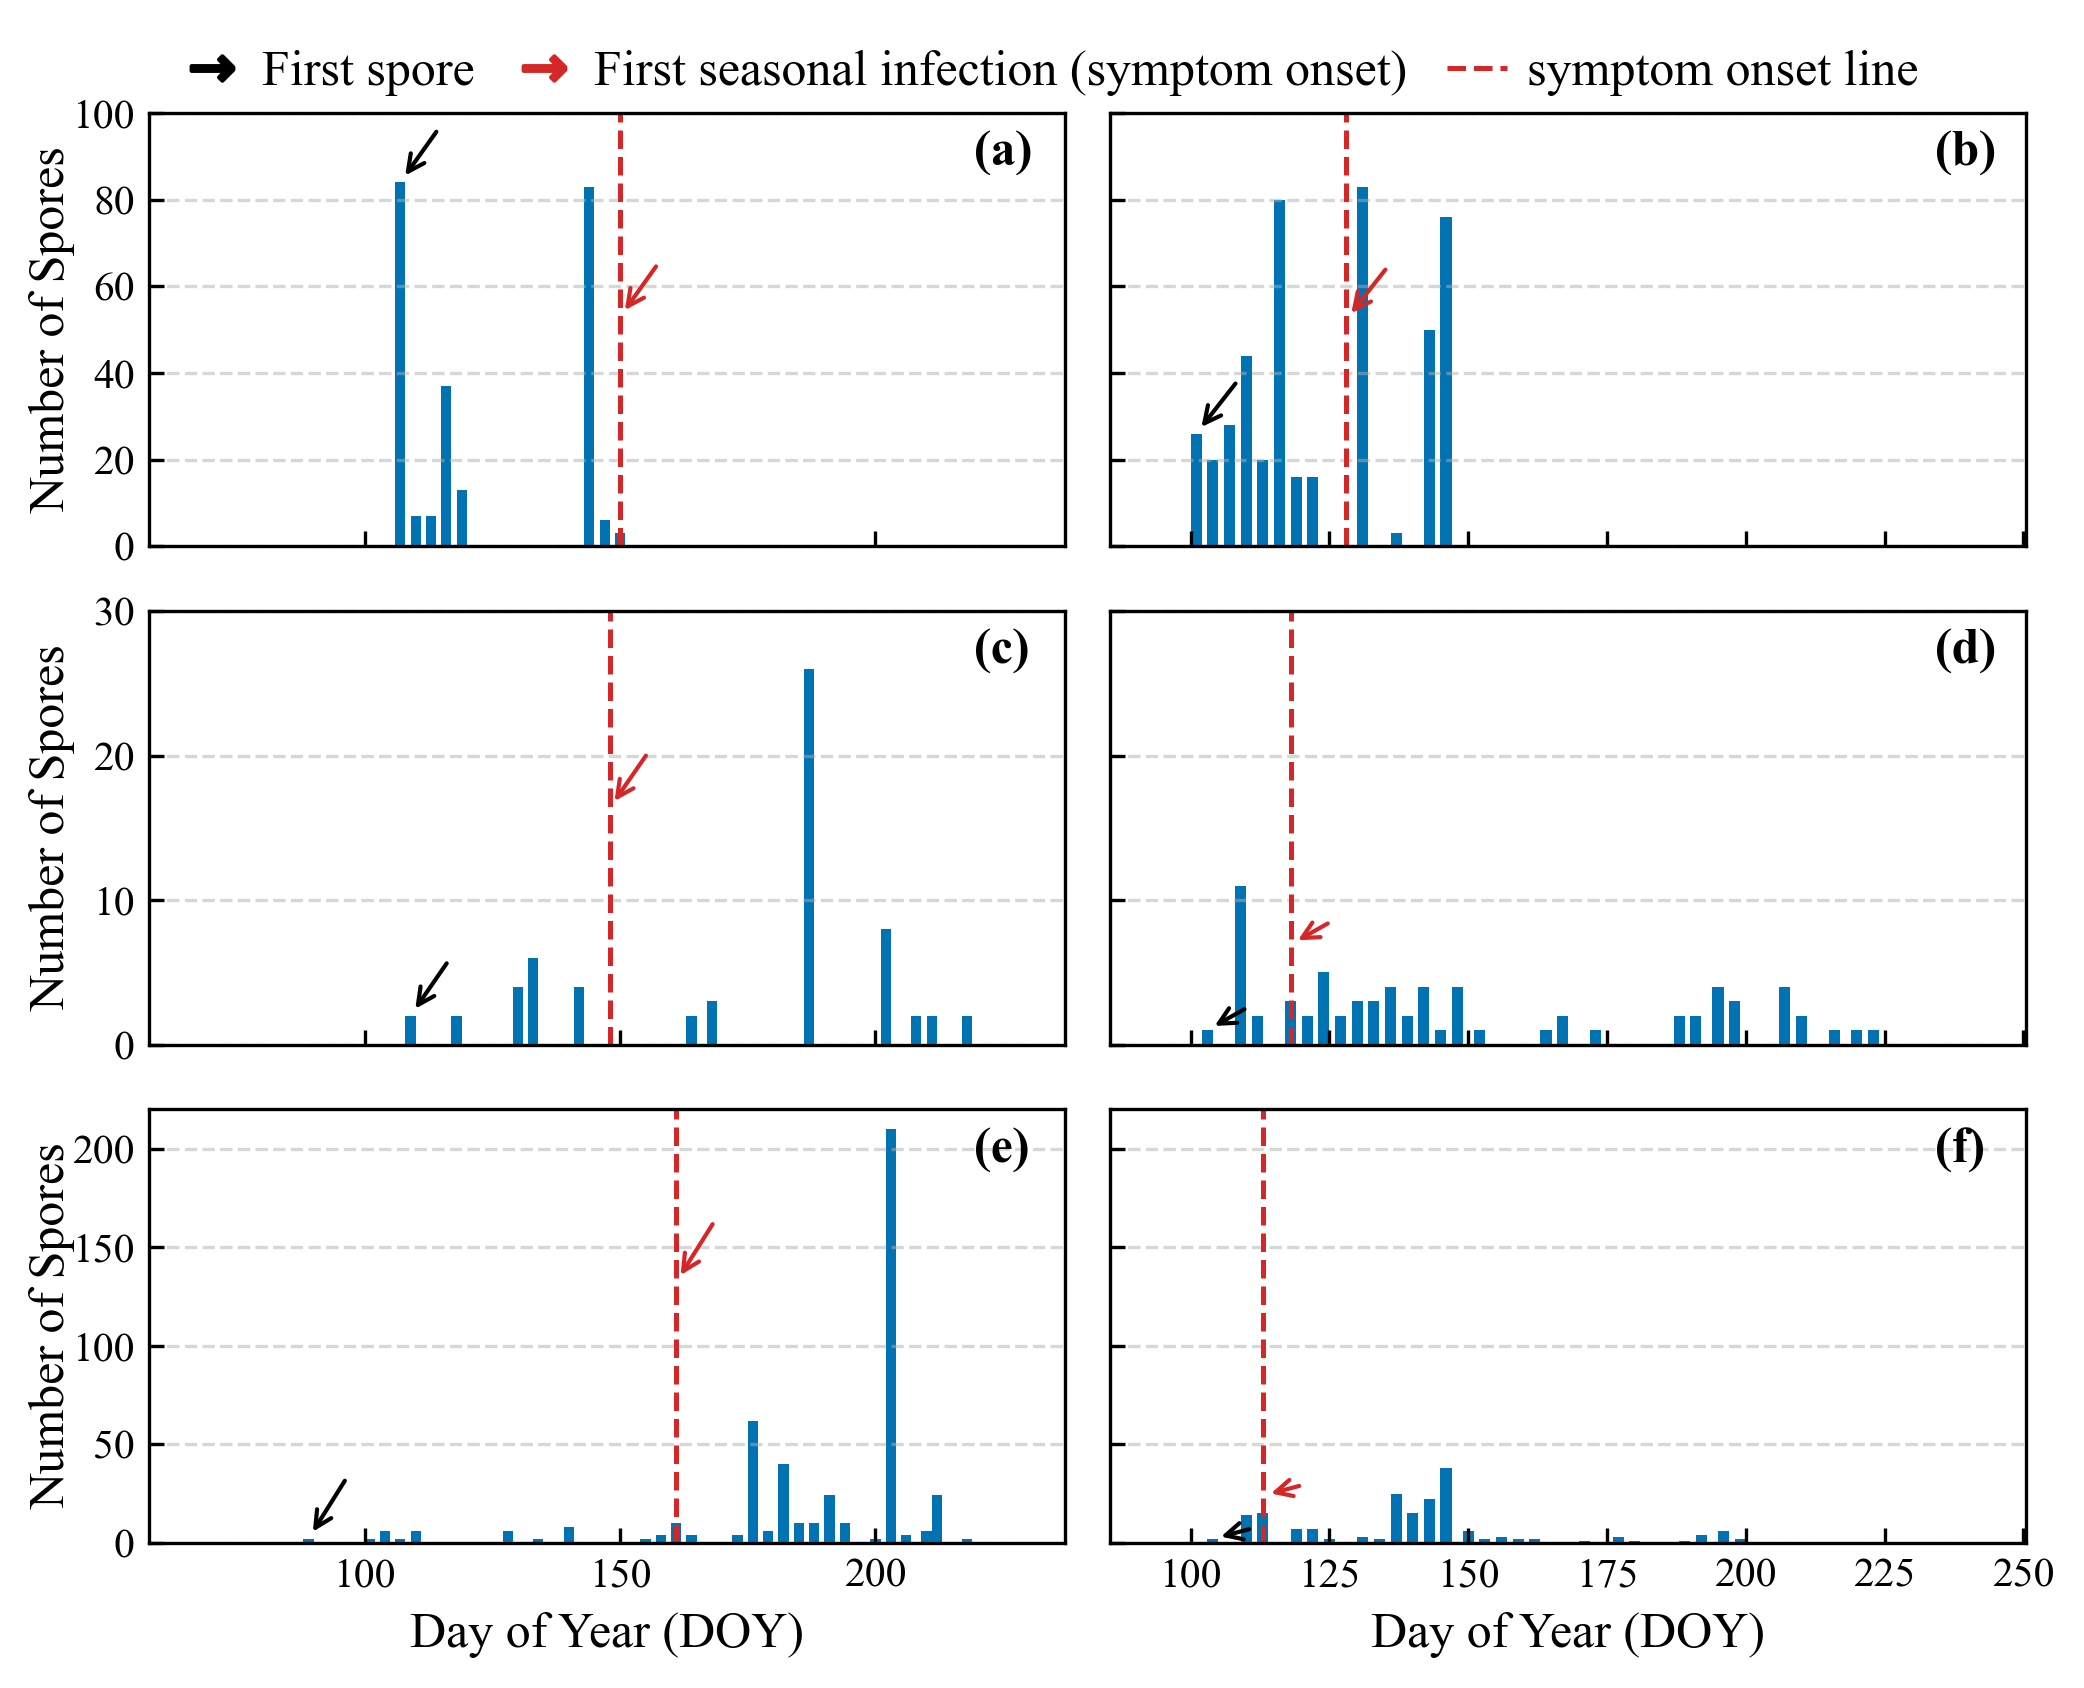
\includegraphics[width=0.95\linewidth]{fig/Figure_08.png}
\caption{Timing of first seasonal infection and sporangia dynamics of
grape downy mildew (\emph{Plasmopara viticola}) in the experimental
vineyard from 2022 to 2024: (a) Guilin, 2022; (b) Hechi, 2022; (c)
Hechi 2023; (d) Hechi, 2024; (e) Nanning, 2023; (f) Nanning, 2024.}
\label{_Ref212492136}
\end{figure}

\subsection{Sensitivity analysis}\label{sensitivity-analysis}

To quantify the relative contribution of model parameters to simulation
outputs and assess the impact of incorporating spore-pressure dynamics,
a global sensitivity analysis was performed using the Morris method.
Parameter influence magnitude and direction were represented by the
absolute mean effect (\(\mu^*\)) and the signed mean effect (\(\mu\)), respectively
(\hyperref[_Ref222510092]{Fig 9}, \hyperref[_Ref222510103]{Fig 10}).

In the baseline FSIM model, ZVPD exhibited the highest sensitivity (\(\mu^*\) =
17.23), followed by DIRM (15.13), TMSO (13.25), and IC (12.67), which
collectively dominated model output (\hyperref[_Ref222510092]{Fig 9a}).

The signed effects revealed distinct directional differentiation: IC
exerted the strongest positive influence (\(\mu = 20.23\)), whereas ZVPD
showed a pronounced negative effect (\(\mu = -20.17\))
(\hyperref[_Ref222510103]{Fig 10a}).

Following the incorporation of spore-pressure dynamics in FSIM-S, the
overall sensitivity ranking remained largely consistent, with ZVPD (\(\mu^*\) =
16.67), DIRM (13.42), IC (13.34), and TMSO (12.93) continuing to rank as
the four most influential parameters (\hyperref[_Ref222510092]{Fig 9b}).
Among the newly introduced spore-related parameters, SAP exhibited
moderate sensitivity (\(\mu^* = 4.63\)), surpassing several existing
environmental and dispersal-related parameters (e.g., STMI, DERM, SMMI),
whereas SAN showed low sensitivity (\(\mu^* = 1.27\)). The signed effects in
FSIM-S (\hyperref[_Ref222510103]{Fig 10b}) maintained similar
directional patterns: IC remained the strongest positive driver
(\(\mu = 18.74\)), ZVPD the strongest negative driver
(\(\mu = -16.59\)), while SAP displayed a clear negative effect
(\(\mu = -7.05\)).

Overall, the sensitivity analysis confirms that the dominant model
drivers remain stable after the incorporation of spore-pressure
dynamics, while the moderate sensitivity of SAP supports the biological
relevance of the spore-pressure formulation in influencing infection
timing.

\begin{figure}[H]
\centering

\includegraphics[width=0.95\linewidth]{fig/Figure_09.png}
\caption{Global parameter sensitivity based on the Morris method
expressed as absolute mean effects (\(\mu^*\)) for the baseline FSIM
model (a) and the extended FSIM-S model incorporating the spore-pressure
formulation (b). Parameters are ranked by decreasing \(\mu^*\),
representing their overall influence magnitude on model output
aggregated across multiple random seeds. Parameter abbreviations: ZVPD =
zoospore\_alive\_\_vpd; DIRM = dispersal\_\_rain\_min; IC =
infection\_\_infection\_condition; TMSO = thresholds\_\_min\_spores;
STMX = sporulation\_\_Tmax; MTWN = mp\_tmp\_\_rh\_wet\_night; DIWM =
dispersal\_\_wind\_min; STOP = sporulation\_\_Topt; STMI =
sporulation\_\_Tmin; ZARA = zoospore\_alive\_\_rain; DERM =
deposition\_\_rain\_min; SMMI = sporulation\_\_MP\_min; ISED =
incubation\_\_spl\_end; SAP = spore\_\_alpha\_pos; SAN =
spore\_\_alpha\_neg. Error bars indicate variability across aggregated
runs.}
\label{_Ref222510092}
\end{figure}

\begin{figure}[H]
\centering

\includegraphics[width=0.95\linewidth]{fig/Figure_10.png}
\caption{Signed mean effects (\(\mu\)) from the Morris global
sensitivity analysis for the baseline FSIM model (a) and the extended
FSIM-S model (b). Positive and negative values indicate the direction of
parameter influence on model output, while bar length reflects effect
magnitude. Results are aggregated across multiple random seeds, with
error bars representing variability among runs.}
\label{_Ref222510103}
\end{figure}

\subsection{Model performance}\label{model-performance}

The predictive performance of FSIM and FSIM-S for first seasonal
infection onset was evaluated using mean absolute error (MAE) and root
mean square error (RMSE) under a three-fold cross-validation framework
(\hyperref[_Ref222858743]{Fig 11}). On the training sets, FSIM achieved
MAE and RMSE values of 6.8 and 8.1 days, respectively, whereas FSIM-S
reduced these to 4.0 and 4.0 days, corresponding to reductions of 41.5\%
and 50.3\%. On the validation sets, FSIM yielded MAE of 9.3 days and
RMSE of 10.6 days, while FSIM-S achieved 6.3 and 6.5 days, representing
reductions of 32.1\% and 38.9\% (\hyperref[_Ref222858743]{Fig 11}).
Notably, FSIM-S also exhibited lower variability across cross-validation
folds, indicating improved predictive stability.

The simulated first seasonal infection onset windows for each site--year
combination are presented in \hyperref[_Ref214273041]{Table 3}. Both
models generally reproduced the observed onset patterns, with FSIM-S
achieving comparable or slightly improved accuracy across most cases.
Errors varied by location and year: the largest deviation occurred in
Guilin 2022, where both models predicted onset approximately 13 days
earlier than observed; in contrast, both models achieved zero error for
Hechi 2023. For Hechi 2022 and Nanning 2023--2024, FSIM-S yielded
smaller temporal deviations than FSIM, while maintaining comparable
prediction windows.

Overall, the incorporation of spore-pressure dynamics into the model
framework resulted in consistent improvements in both prediction
accuracy and stability, with FSIM-S outperforming FSIM across training
and validation datasets and demonstrating enhanced precision across
site--year combinations.

\protect\phantomsection\label{_Ref214273041}{}
\begin{center}
\textbf{Table 3} Simulated first seasonal infection onset windows and
corresponding deviations (Error) from observed symptom appearance across
sites and years for FSIM and FSIM-S. Negative Error values indicate that
the simulated onset occurred earlier than observed. ``Simulated Onset''
denotes the model-estimated oil-spot appearance window representing
first seasonal infection expression. Results shown correspond to the
final global parameter configuration selected from cross-validation
folds (see Section 2.5.4).
\end{center}

{\def\LTcaptype{none} % do not increment counter
\begin{longtable}[]{@{}
  >{\raggedright\arraybackslash}p{(\linewidth - 8\tabcolsep) * \real{0.1537}}
  >{\raggedright\arraybackslash}p{(\linewidth - 8\tabcolsep) * \real{0.1706}}
  >{\raggedright\arraybackslash}p{(\linewidth - 8\tabcolsep) * \real{0.1366}}
  >{\raggedright\arraybackslash}p{(\linewidth - 8\tabcolsep) * \real{0.3126}}
  >{\raggedright\arraybackslash}p{(\linewidth - 8\tabcolsep) * \real{0.2264}}@{}}
\toprule\noalign{}
\begin{minipage}[b]{\linewidth}\raggedright
Model
\end{minipage} & \begin{minipage}[b]{\linewidth}\raggedright
Site
\end{minipage} & \begin{minipage}[b]{\linewidth}\raggedright
Year
\end{minipage} & \begin{minipage}[b]{\linewidth}\raggedright
Simulated Onset (Month-Day)
\end{minipage} & \begin{minipage}[b]{\linewidth}\raggedright
Error (days)
\end{minipage} \\
\midrule\noalign{}
\endhead
\bottomrule\noalign{}
\endlastfoot
FSIM & Guilin & 2022 & May 15--17 & -13.0 \\
& Hechi & 2022 & May 14--15 & +6.0 \\
& Hechi & 2023 & May 28--30 & +0.0 \\
& Hechi & 2024 & Apr 25--26 & -1.0 \\
& Nanning & 2023 & Jun 15--16 & +5.0 \\
& Nanning & 2024 & Apr 25--26 & +3.0 \\
FSIM-S & Guilin & 2022 & May 15--17 & -13.0 \\
& Hechi & 2022 & May 13--14 & +5.0 \\
& Hechi & 2023 & May 28--29 & +0.0 \\
& Hechi & 2024 & Apr 24--25 & -2.0 \\
& Nanning & 2023 & Jun 14--15 & +4.0 \\
& Nanning & 2024 & Apr 24--25 & +2.0 \\
\end{longtable}
}

\begin{figure}[H]
\centering
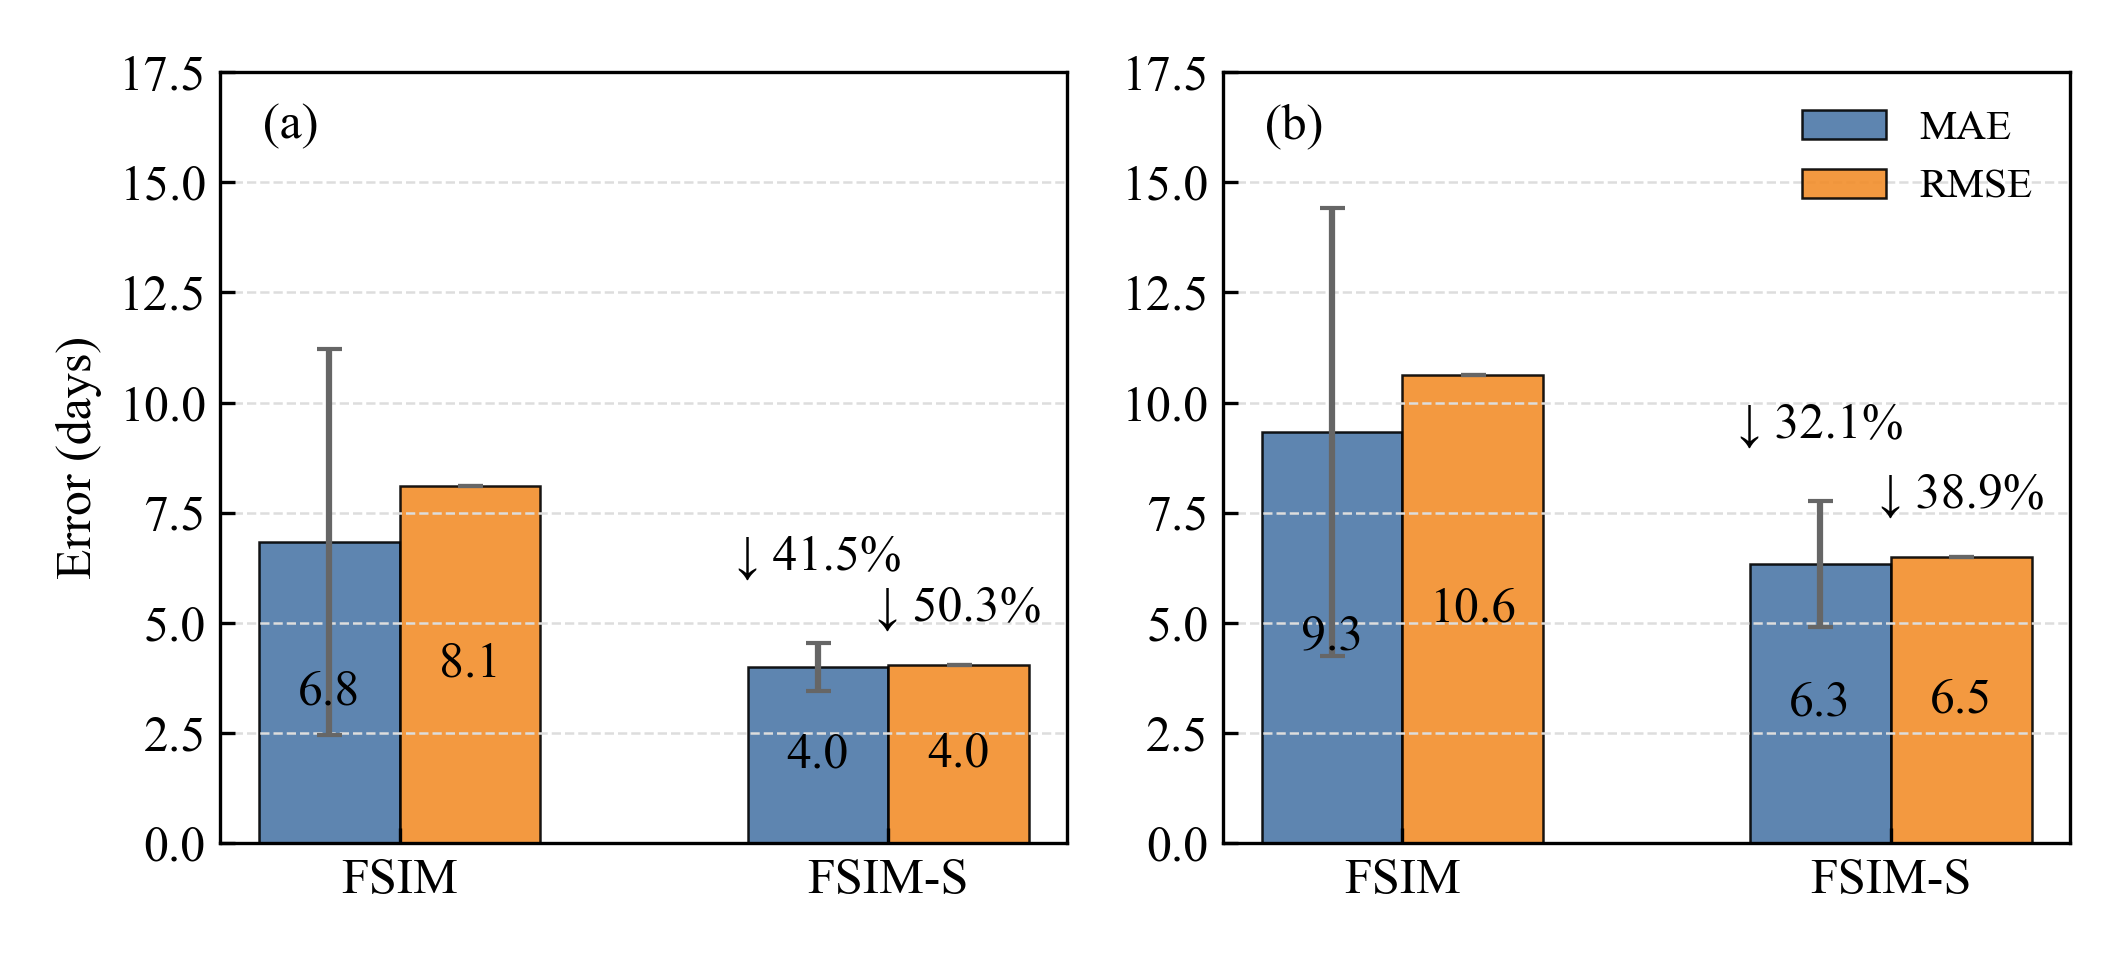
\includegraphics[width=0.95\linewidth]{fig/Figure_11.png}
\caption{Model performance comparison based on mean absolute error
(MAE) and root mean square error (RMSE): (a) training set and (b) test
set. Bars show mean errors (days) ± standard deviations across folds.
The percentages denote relative error reductions compared with the
baseline FSIM model.}
\label{_Ref222858743}
\end{figure}

\subsection{Spatial distribution of first-infection onset across Guangxi
(2000--2024)}\label{spatial-distribution-of-first-infection-onset-across-guangxi-2000-2024}

Based on historical ERA5 meteorological data, the spatial distribution
of first-infection onset across Guangxi from 2000 to 2024 was
reconstructed using FSIM-S, simulated under three variety-specific
phenology scenarios: Wink (WK), Kyoho (JF), and Yeniang No. 2 (MPT)
(\hyperref[_Ref223011563]{Fig 12}).

Multi-year mean onset dates were similar across varieties, with WK and
JF averaging DOY 195 and MPT DOY 198 (median: 196, 196, and 199,
respectively). Spatially, earlier onset dates were consistently
simulated in central--southern and parts of southwestern Guangxi,
whereas later onset occurred in northern and northeastern areas
(\hyperref[_Ref223011563]{Fig 12a--c}). This spatial gradient was
consistent across all three varieties.

Frequency distributions (\hyperref[_Ref223011563]{Fig 12d}) showed that
the majority of onset dates fell within DOY 180--210 across all
varieties, with peak frequencies concentrated around DOY 190--200. The
overall distribution structures were highly similar among varieties.

\begin{figure}[H]
\centering
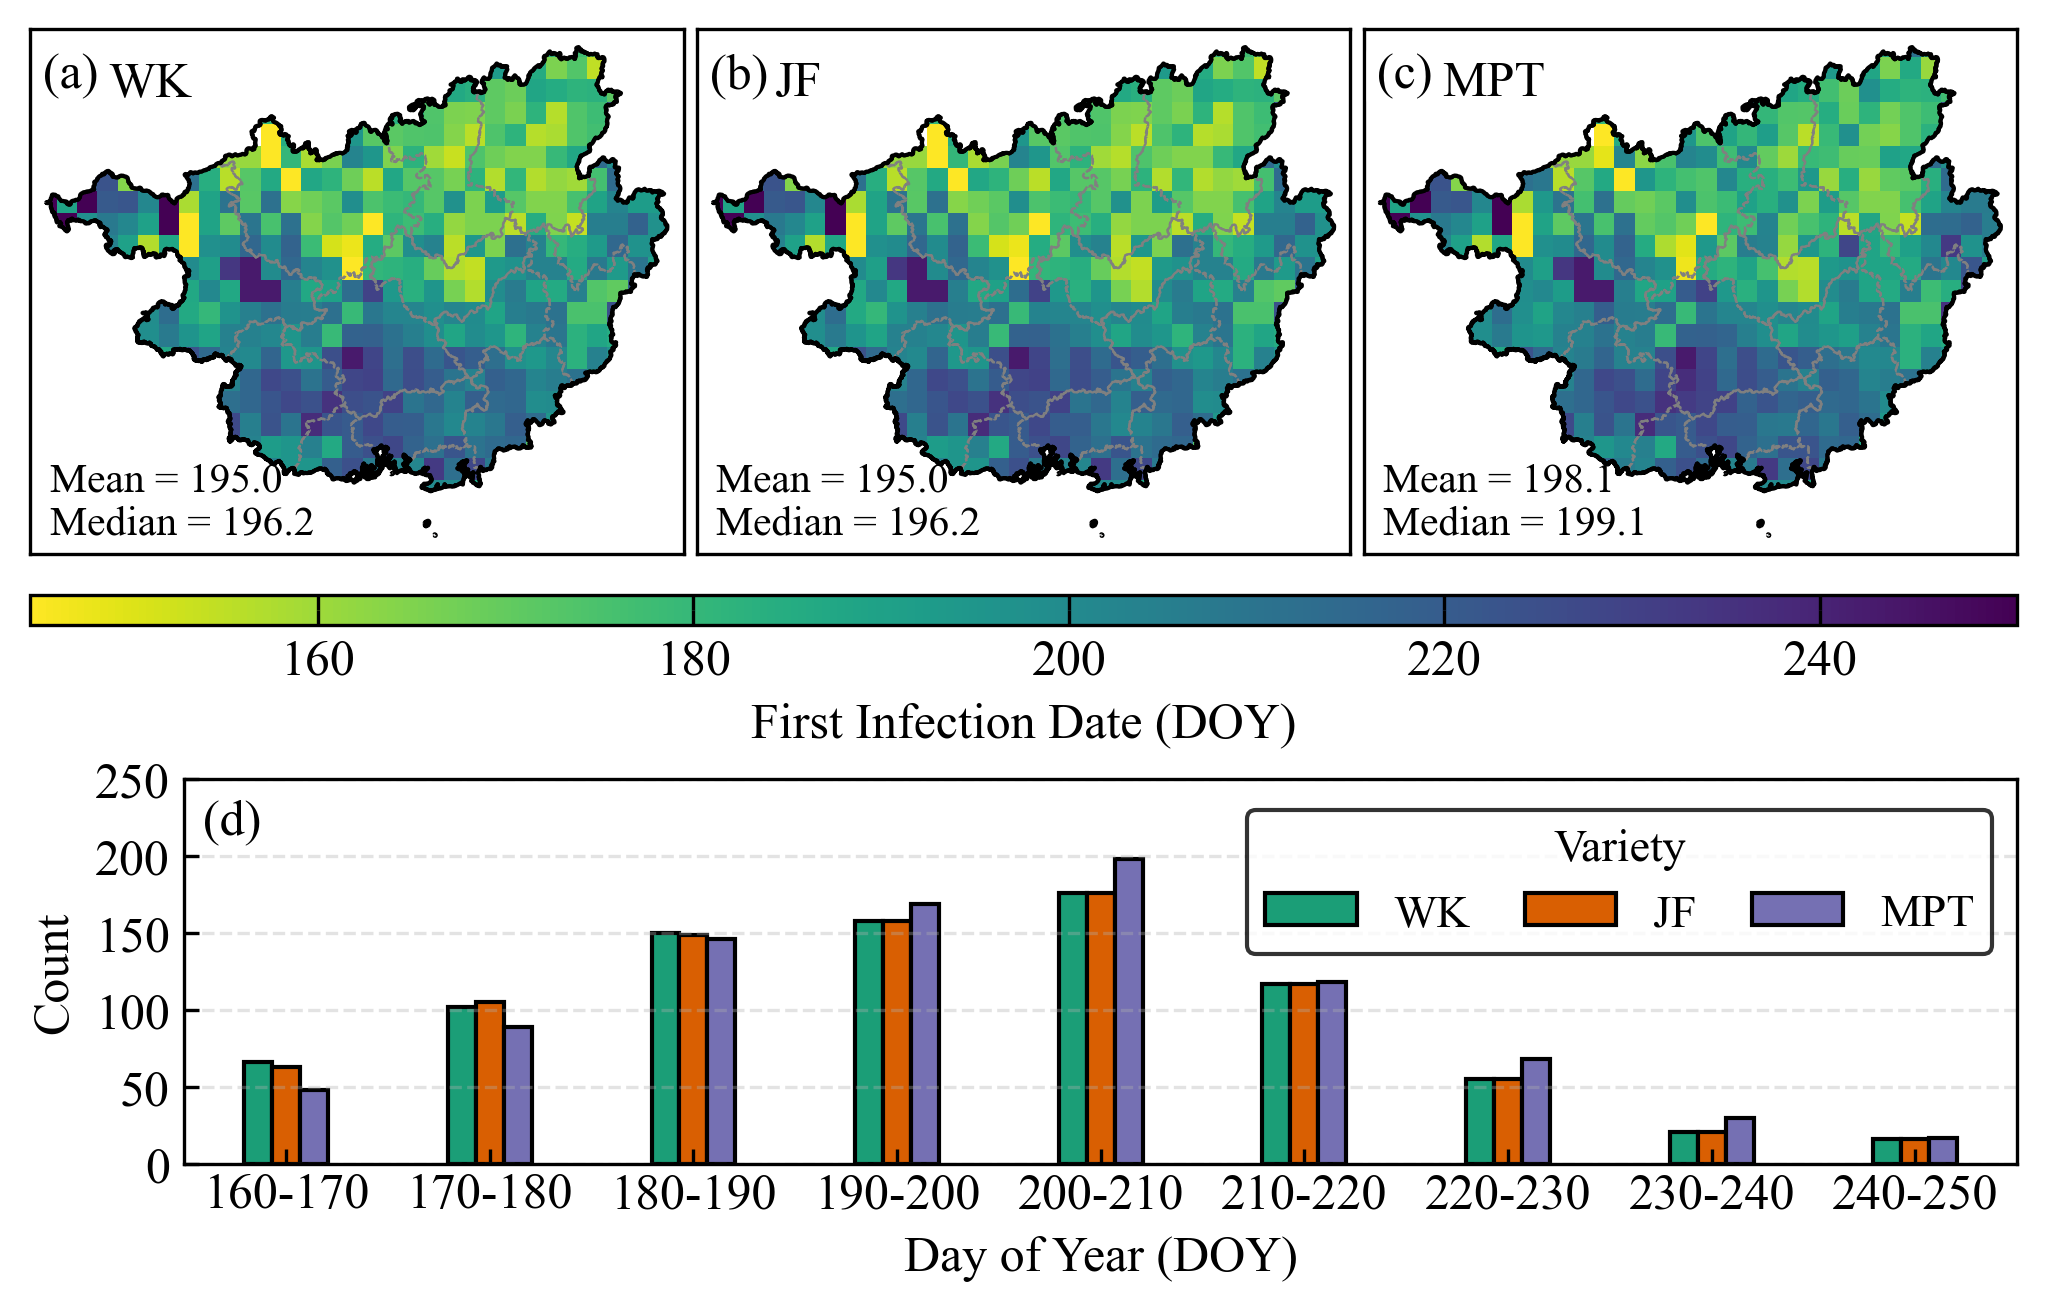
\includegraphics[width=0.95\linewidth]{fig/Figure_12.png}
\caption{Simulated mean onset dates (day of year, DOY) of first
seasonal infection under the FSIM-S model for three varieties: (a--c)
spatial distributions of the Wink (WK), Kyoho (JF), and Yeniang No. 2
(MPT), and (d) their DOY frequency distributions.}
\label{_Ref223011563}
\end{figure}

\subsection{Regional disease-management implications
(2000--2024)}\label{regional-disease-management-implications-2000-2024}

The potential to improve early disease-management timing across Guangxi
from 2000 to 2024 was evaluated by comparing the FSIM-S-derived timing of
first seasonal infection with a representative conventional fixed
calendar programme (\hyperref[_Ref223012659]{Fig 13}). Across the three
grapevine varieties, the model-guided strategy identified approximately
three potentially avoidable early preventive applications per season on
average (mean: 3.0 sprays; median: 2.7 sprays), with minimal variation
among varieties. This result indicates that the main management value of
FSIM-S lies in delaying unnecessary pre-risk sprays while retaining
protection near the simulated infection window.

Spatially, higher saving potential was concentrated in central--southern
and southwestern Guangxi, where simulated first-infection onset tended
to occur later relative to the representative calendar programme, whereas
northern and northeastern areas showed relatively lower savings
(\hyperref[_Ref223012659]{Fig 13a--c}). This spatial pattern was
consistent across all three varieties.

The frequency distribution (\hyperref[_Ref223012659]{Fig 13d}) showed
that spray savings were predominantly two to four applications per
season, with two or three sprays being the most common. Higher savings
(\(\geq\)5 sprays) occurred less frequently but were present in certain
locations. The overall distribution structures were highly similar among
varieties, suggesting that spatial climatic variability exerted a
stronger influence on early-season management timing than the simplified
variety scenarios considered here.

\begin{figure}[H]
\centering
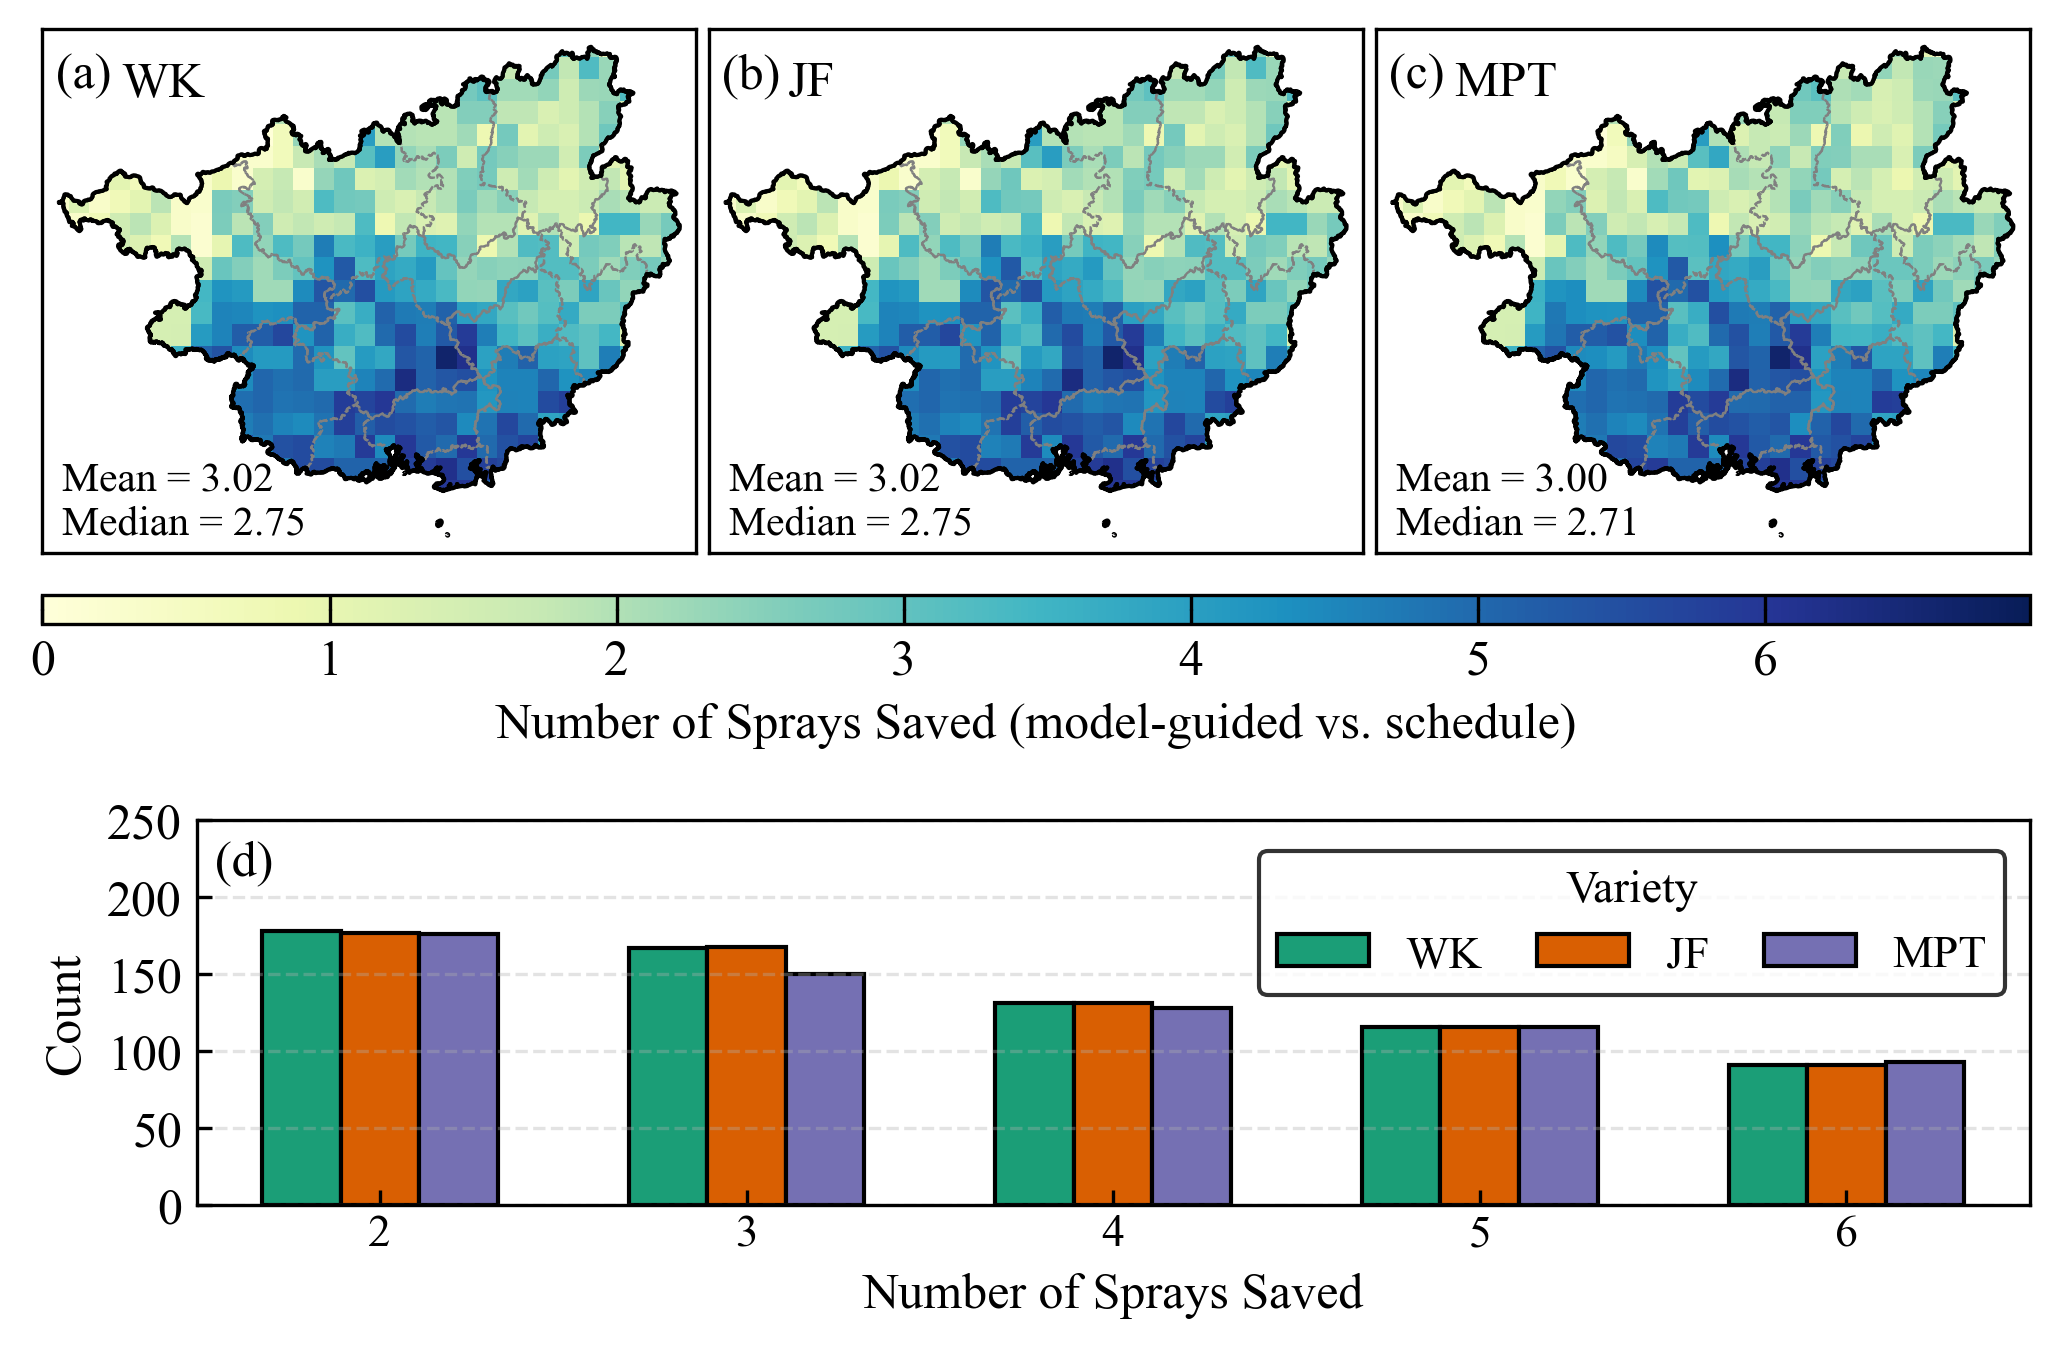
\includegraphics[width=0.95\linewidth]{fig/Figure_13.png}
\caption{Spatial distribution and frequency of model-guided spray
savings under the FSIM-S model: (a--c) multi-year mean number of sprays
saved per grid cell for the Wink (WK), Kyoho (JF), and Yeniang No. 2
(MPT), and (d) frequency distribution of spray savings.}
\label{_Ref223012659}
\end{figure}

\section{Discussion}\label{discussion}

This study addressed a key agronomic challenge in subtropical
viticulture: improving early-season grapevine downy mildew management
when viable inoculum may be present before weather and crop conditions
become jointly favourable for infection. By reconstructing Rossi's
primary and secondary infection formulations into a First Seasonal
Infection Model (FSIM), and then incorporating observation-based
spore-pressure dynamics (FSIM-S), the study linked on-farm inoculum
monitoring with agroclimatic process modelling.

Across multiple site--year datasets from Guangxi, China, FSIM-S
improved prediction accuracy and stability compared with FSIM while
retaining the dominant influence of meteorological drivers. These
results support the use of FSIM-S as a region-adapted mechanistic
framework for field-based downy mildew decision support in subtropical
vineyards, rather than as an empirical model fitted only to symptom
dates.

\subsection{Inoculum dynamics and the drivers of first seasonal
infection
timing}\label{inoculum-dynamics-and-the-drivers-of-first-seasonal-infection-timing}

In temperate systems, seasonal epidemics are typically initiated by
overwintering oospores after a distinct climatic break. In contrast, the
continuous presence of airborne sporangia during the early growing
season (\hyperref[_Ref214187767]{Fig 5}, \hyperref[_Ref212492136]{Fig
8}) indicates that inoculum in the studied subtropical vineyards is not
restricted to a discrete primary infection event. This distinction has
direct implications for model structure, because frameworks centred on
oospore-driven primary infection may not fully represent systems in
which asexual inoculum is recurrently available.

Despite this continuous inoculum presence, the timing of first seasonal
infection varied substantially across sites and years
(\hyperref[_Ref212492136]{Fig 8}). This variability is consistent with
interannual differences in early-season meteorological conditions.
Temperature, relative humidity, and leaf wetness duration regulate
infection initiation (Rossi and Caffi, 2012; Yi et al., 2019; Yu et
al., 2022), whereas sustained rainfall can promote sporangial
production, release and dispersal from vineyard inoculum sources
(Orlandini et al., 2008). Accordingly, climate variability affects
disease onset through both infection suitability and inoculum dynamics,
explaining why first seasonal infection cannot be inferred from weather
suitability alone.

The temporal decoupling between sporangia detection and symptom onset
provides further evidence for this interpretation. Across all datasets,
the interval between first airborne sporangia detection and subsequent
symptom appearance ranged from 9 to 72 days
(\hyperref[_Ref212492136]{Fig 8}), indicating that the presence of
inoculum is necessary but insufficient for successful infection.
Infection establishment depends also on host phenological susceptibility
(Hui et al., 2022) and on sufficient inoculum pressure to support
effective deposition and infection (Scholthof, 2007; Van der Plank,
2013; Zhang et al., 2025). This decoupling indicates that inoculum
pressure should be represented as a dynamic constraint on infection
triggering, rather than treated as a static prerequisite.

\subsection{Model enhancement and evidence from sensitivity
analysis}\label{model-enhancement-and-evidence-from-sensitivity-analysis}

The incorporation of spore-pressure dynamics into FSIM-S improved
predictive performance relative to the baseline FSIM, with validation
MAE reduced to 6.3 days (32\% reduction) (\hyperref[_Ref222858743]{Fig
11}). The improvement suggests that first seasonal infection tends to
occur within comparatively narrow windows in which environmental
suitability coincides with sufficient pathogen pressure, consistent with
the disease triangle concept (Van der Plank, 2013). The model therefore
adds process information beyond weather-only infection suitability while
retaining direct biological interpretability.

Simulations using the final global parameter configuration revealed
site-specific performance patterns (\hyperref[_Ref214273041]{Table 3}).
The larger deviation in Guilin occurred in the single available season
for that site and may reflect local epidemiological conditions that were
less represented in the calibration dataset. By contrast, the stable
multi-year performance in Hechi---including zero error in 2023---shows
that FSIM-S can reproduce infection timing when observations provide
adequate constraints on the relationship between inoculum dynamics and
weather suitability (Yi et al., 2019). In Nanning, the modest positive
bias in 2023--2024 suggests that local microclimate, cultivation
practices, or cultivar resistance may further refine model transfer
across sites (Kiefer et al., 2002; Gessler et al., 2011).

Sensitivity analysis clarified the relative contribution of model
drivers (\hyperref[_Ref222510092]{Fig 9},
\hyperref[_Ref222510103]{Fig 10}). In both models, moisture-related
conditions (ZVPD) exerted the strongest negative influence, reflecting
the critical role of humidity in zoospore release and leaf surface
wetness (Yu et al., 2021; Hui et al., 2023). In
FSIM-S, the newly introduced spore-pressure regulation parameter SAP
exhibited a moderate negative directional effect, indicating that higher
inoculum pressure facilitates earlier attainment of infection thresholds
(Brischetto et al., 2021). Notably, SAP did not alter the dominant
sensitivity ranking of environmental drivers, suggesting that inoculum
pressure acts primarily as an infection-trigger amplifier rather than
replacing meteorological drivers.

Overall, FSIM provides a mechanistic representation of first seasonal
infection processes in subtropical vineyards where recurrent sporangia
production is a major inoculum source. FSIM-S further integrates an
observation-derived spore-pressure field, improving responsiveness to
infection timing variability while preserving the core biological
processes inherited from mechanistic infection modelling. This balance
between biological structure and field observation is important for
developing transferable early-warning tools under variable subtropical
conditions.

\subsection{Agronomic implications for climate-smart vineyard disease
management}\label{agronomic-implications-for-climate-smart-vineyard-disease-management}

The regional simulations provide an agronomic interpretation of when
model-guided protection would be most relevant across Guangxi. FSIM-S
predicted a mean first-infection onset between DOY 195 and 198, with a
high-frequency window spanning DOY 180--210
(\hyperref[_Ref223011563]{Fig 12}). This period overlaps with the
regional flowering--fruit-set stage, when young tissues are particularly
susceptible (Wang et al., 2020; Cheng et al., 2022), and with the Meiyu
season, characterized by warm, humid conditions and intermittent
rainfall (Song et al., 2021; Tian et al., 2022). Thus, the regional
results are not only spatial reconstructions of infection timing; they
also identify the seasonal context in which downy mildew decisions are
most consequential for vineyard production.

Within this context, the management implication of FSIM-S is to
translate infection biology and agroclimatic variability into a
time-explicit risk signal. This signal can support decisions on early
scouting, spore monitoring intensity, protection timing and chemical
intervention. When model outputs were compared with conventional
calendar-based programmes, the model-guided scenario avoided an average
of approximately three early preventive sprays per season (range:
2--5), equivalent to a 20--50\% reduction in the simulated early-season
programme (Gisi and Sierotzki, 2008; Rossi et al., 2008; Rossin et al.,
2015; Koledenkova et al., 2022). This result should be interpreted as a
timing benefit rather than as a generic fungicide-reduction claim: the
model delays pre-risk sprays while retaining protection near the
simulated infection window.

The climate-smart value of this framework therefore lies in shifting
subtropical downy mildew management from fixed calendar schedules toward
risk-informed decision support. FSIM-S does not imply that early
protection can be omitted; rather, it identifies periods when host
susceptibility, spore-pressure dynamics and agroclimatic suitability
converge. Such information can improve the biological justification of
interventions, increase pesticide-use efficiency, and support more
sustainable viticulture under humid subtropical conditions (Russell,
1995; Zubrod et al., 2019; Zhang et al., 2020).

\subsection{Limitations and future
directions}\label{limitations-and-future-directions}

First, model parameterization used observations from two commercial
vineyards and one experimental orchard over three growing seasons. This
provides multi-site and multi-year evidence under realistic subtropical
production conditions, while additional observations across more
regions, cultivars and management systems would further broaden the
calibration domain. The 2022 Guilin season, for example, provided a
useful contrast because unusually low early-season humidity and
irregular rainfall (\hyperref[_Ref214271335]{Fig 3}) may have delayed
or suppressed infection establishment. Such contrasting cases are
valuable for testing model behaviour, but wider datasets would support
more explicit cultivar- or region-specific parameterization (Bellin et
al., 2009; Gessler et al., 2011; Koledenkova et al., 2022).

Second, FSIM-S currently uses a deterministic mechanistic structure to
describe the coupling between meteorological conditions and
spore-pressure dynamics. This formulation favours stability,
interpretability and transparent biological assumptions at the regional
scale. Future probabilistic extensions could complement this structure
by quantifying uncertainty associated with rainfall variability, spore
sampling error and fine-scale atmospheric heterogeneity, particularly
when the model is applied to operational warning systems or climate
scenario analysis.

Finally, the regional analysis was designed as a scenario-based
assessment rather than a vineyard-by-vineyard operational map. It
therefore used simplified assumptions about vineyard distribution,
canopy structure and cultivar allocation. These assumptions are
appropriate for evaluating broad regional patterns and management
windows, but finer-scale implementation would benefit from vineyard
land-use layers, cultivar distribution data, remote-sensing information
and canopy microclimate observations (Tesic et al., 2007; Perria et
al., 2022). Such additions would extend the framework from regional risk
assessment toward more spatially resolved disease-management support.

\section{Conclusion}\label{conclusion}

This study developed FSIM-S, a spore-informed and process-based
agroclimatic modelling framework for timing grapevine downy mildew
management under subtropical conditions. By incorporating
field-observed sporangia data through a dynamic spore-pressure field,
the model links inoculum dynamics, dispersal processes and
meteorological drivers within a field-tested decision-support framework.
Multi-year and multi-site validation demonstrated that FSIM-S reproduced
first seasonal infection timing with a mean absolute error of 6.3 days
and a root mean square error of 6.5 days. Long-term regional simulations
(2000--2024) captured realistic spatial patterns of infection onset and
indicated that model-guided timing could avoid 2--5 early preventive
sprays per season compared with a conventional calendar-based programme.
Overall, FSIM-S provides a
data-integrated basis for climate-smart, model-guided disease management
and more sustainable fungicide use in subtropical viticulture.

\section{CRediT authorship contribution
statement}\label{credit-authorship-contribution-statement}

Linjia Yao: Investigation, Writing -- original draft, Visualization,
Software, Methodology, Formal analysis, Conceptualization. Bin Chen:
Investigation, Writing -- original draft, Formal analysis. Writing
-review \& editing. Vittorio Rossi: Formal analysis, Writing -review \&
editing. Ling Yin: Funding acquisition, Writing -review \& editing.
Shumei Wei: Investigation. Qi Tian: Investigation. Changqing Yan:
Writing -review \& editing. Hui Wang: Writing -review \& editing.
Antonio Fernandes Nogueira Júnior: Writing -review \& editing. Yu Huang:
Investigation. Qiang Yu: Conceptualization, Supervision. Junjie Qu:
Funding acquisition. Gang Zhao: Software, Methodology,
Conceptualization, Supervision.

\section{Declaration of competing
interest}\label{declaration-of-competing-interest}

The authors declare that they have no known competing financial
interests or personal relationships that could have appeared to
influence the work reported in this paper.

\section{Acknowledgements}\label{acknowledgements}

This work was funded by Guangxi Key R\&D Program Project (Grant No. Gui
Ke AB24010121, AB21076001) and the Key Research and Development Program
of Shaanxi (Grant No. 2023-ZDLNY-64). We gratefully acknowledge Mr. Yunlong Chen and Mr.
Yaokang Liang, local growers in Guilin and Hechi, for their valuable
assistance in fieldwork.

\section{Data Availability}\label{data-availability}

The model structure, code, and data supporting the findings of this
study are publicly available at:
\url{https://github.com/SmartAG-Team/grape_disease.git}. The repository
includes (i) field observations of first seasonal infection (symptom
onset), (ii) airborne sporangia monitoring data, (iii) site--year
meteorological data used for model calibration and validation, and (iv)
code for model implementation, calibration, and figure generation.
Additional materials may be available from the corresponding author upon
reasonable request (\ul{gang.zhao@nwafu.edu.cn (Gang Zhao)}).

\section{References}\label{references}

Baldacci, E., 1947. Epifitie di Plasmopara viticola (1941-46)
nell'oltrepò pavese ed adizione del calendario di incubazione come
strumento di lotta.

Barrett, J., 1939. Overwintering mycelium of Plasmopara viticola (B. \&
C.) Berl. \& de T. in the California wild grape, Vitis californica
Benth.

Bellin, D., Peressotti, E., Merdinoglu, D., Wiedemann-Merdinoglu, S.,
Adam-Blondon, A.-F., Cipriani, G., Morgante, M., Testolin, R., Di
Gaspero, G., 2009. Resistance to Plasmopara viticola in grapevine
`bianca' is controlled by a major dominant gene causing localised
necrosis at the infection site. Theor. Appl. Genet. 120, 163--176.
https://doi.org/10.1007/s00122-009-1167-2

Bergstra, J., Bardenet, R., Bengio, Y., Kégl, B., 2011. Algorithms for
hyper-parameter optimization, in: Advances in Neural Information
Processing Systems 24. Curran Associates, Inc.

Brischetto, C., Bove, F., Fedele, G., Rossi, V., 2021. A weather-driven
model for predicting infections of grapevines by sporangia of Plasmopara
viticola. Front. Plant Sci. 12, 636607.
https://doi.org/10.3389/fpls.2021.636607

Caffi, T., Rossi, V., Bugiani, R., 2010. Evaluation of a warning system
for controlling primary infections of grapevine downy mildew. Plant Dis.
94, 709--716. https://doi.org/10.1094/PDIS-94-6-0709

Caffi, T., Rossi, V., Cossu, A., Fronteddu, F., 2007. Empirical vs.
mechanistic models for primary infections of \emph{Plasmopara viticola}
*. EPPO Bull. 37, 261--271.
https://doi.org/10.1111/j.1365-2338.2007.01120.x

Carisse, O., 2016. Development of grape downy mildew (plasmopara
viticola) under northern viticulture conditions: Influence of fall
disease incidence. Eur. J. Plant Pathol. 144, 773--783.
https://doi.org/10.1007/s10658-015-0748-y

Carisse, O., Van Der Heyden, H., Tremblay, D.M., Hébert, P.O., Delmotte,
F., 2021. Evidence for differences in the temporal progress of
\emph{Plasmopara viticola} Clades \emph{riparia} and \emph{aestivalis}
airborne inoculum monitored in vineyards in eastern Canada using a
specific multiplex quantitative PCR assay. Plant Dis. 105, 1666--1676.
https://doi.org/10.1094/PDIS-06-20-1164-RE

Chavas, J., Nauges, C., 2020. Uncertainty, Learning, and Technology
Adoption in Agriculture. Appl. Econ. Perspect. Policy 42, 42--53.
https://doi.org/10.1002/aepp.13003

Chen, M., Brun, F., Raynal, M., Makowski, D., 2019. Timing of grape
downy mildew onset in Bordeaux vineyards. Phytopathology 109, 787--795.
https://doi.org/10.1094/PHYTO-12-17-0412-R

Chen, M., Brun, F., Raynal, M., Makowski, D., 2020. Forecasting severe
grape downy mildew attacks using machine learning. PLOS ONE 15,
e0230254. https://doi.org/10.1371/journal.pone.0230254

Cheng, X., Sun, S., Liu, Z., Yang, X., 2022. Drought analysis during the
growth stages of grape in the main grape-growing regions in China.
Theor. Appl. Climatol. 149, 1497--1507.
https://doi.org/10.1007/s00704-022-04070-z

García-Esparza, M., Capri, E., Pirzadeh, P., Trevisan, M., 2006. Copper
content of grape and wine from Italian farms. Food Addit. Contam. 23,
274--280. https://doi.org/10.1080/02652030500429117

Gessler, C., Pertot, I., Perazzolli, M., 2011. Plasmopara viticola: A
review of knowledge on downy mildew of grapevine and effective disease
management. Phytopathol. Mediterr. 50, 3--44.
https://www.jstor.org/stable/26458675

Gisi, U., Sierotzki, H., 2008. Fungicide modes of action and resistance
in downy mildews. Eur. J. Plant Pathol. 122, 157--167.
https://doi.org/10.1007/s10658-008-9290-5

Gobbin, D., Jermini, M., Loskill, B., Pertot, I., Raynal, M., Gessler,
C., 2005. Importance of secondary inoculum of \emph{Plasmopara viticola}
to epidemics of grapevine downy mildew. Plant Pathol. 54, 522--534.
https://doi.org/10.1111/j.1365-3059.2005.01208.x

Gobbin, D., Rumbou, A., Linde, C.C., Gessler, C., 2006. Population
genetic structure of \emph{Plasmopara viticola} after 125 years of
colonization in European vineyards. Mol. Plant Pathol. 7, 519--531.
https://doi.org/10.1111/j.1364-3703.2006.00357.x

Hersbach, H., Bell, B., Berrisford, P., Hirahara, S., Horányi, A.,
Muñoz-Sabater, J., Nicolas, J., Peubey, C., Radu, R., Schepers, D.,
Simmons, A., Soci, C., Abdalla, S., Abellan, X., Balsamo, G., Bechtold,
P., Biavati, G., Bonavita, M., et al., 2020. The ERA5 global reanalysis.
Q. J. R. Meteorol. Soc. 146, 1999--2049. https://doi.org/10.1002/qj.3803

Hill, G., 1990. Plasmopara risk oppenheim--a deterministic computer
model for the viticultural extension service. Not. Sulle Mal. Delle
Piante 111, 231--238.

Huffman, W.E., 2020. Human capital and adoption of innovations: Policy
implications. Appl. Econ. Perspect. Policy 42, 92--99.
https://doi.org/10.1002/aepp.13010

Hug, F., 2005. Genetic structure and epidemiology of Plasmopara viticola
populations from Australian grape-growing regions 54 S.
https://doi.org/10.3929/ETHZ-A-004997559

Hui, W., Shuyi, Y., Wei, Z., Junbo, P., Haiyun, T., Chunhao, L., Jiye,
Y., 2023. Modeling the dynamic changes in Plasmopara viticola sporangia
concentration based on LSTM and understanding the impact of relative
factor variability. Int. J. Biometeorol. 67, 993--1002.
https://doi.org/10.1007/s00484-022-02419-7

Hui, W., Wei, Z., Bregaglio, S., Shuyi, Y., Xinghong, L., Yonghua, L.,
Chunhao, L., Jiye, Y., 2022. Adoption of Sobol's analysis method
improved the application of a coupled primary and secondary infection
grape downy mildew model in northern China. Comput. Electron. Agric.
199, 107154. https://doi.org/10.1016/j.compag.2022.107154

Iooss, B., Lemaître, P., 2015. A review on global sensitivity analysis
methods. Uncertain. Manag. Simul.-Optim. Complex Syst. Algorithms Appl.
101--122. https://doi.org/10.1007/978-1-4899-7547-8\_5

Kiefer, B., Riemann, M., Büche, C., Kassemeyer, H.-H., Nick, P., 2002.
The host guides morphogenesis and stomatal targeting in the grapevine
pathogen Plasmopara viticola. Planta 215, 387--393.
https://doi.org/10.1007/s00425-002-0760-2

Killigrew, B., Sivasithamparam, K., Scott, E., 2005. Absence of oospores
of downy mildew of grape caused by Plasmopara viticola as the source of
primary inoculum in most Western Australian vineyards. Plant Dis. 89,
777. https://doi.org/10.1094/PD-89-0777C

Kocsis, I., Petróczy, M., Markó, G., 2024. Bridging boundaries:
Exploring vineyard, management and variety characteristics influencing
long-term infection of grapevine pathogens. OENO One 58.
https://doi.org/10.20870/oeno-one.2024.58.1.7677

Koledenkova, K., Esmaeel, Q., Jacquard, C., Nowak, J., Clément, C., Ait
Barka, E., 2022. Plasmopara viticola, the causal agent of downy mildew of
grapevine: From its taxonomy to disease management. Front. Microbiol.
13, 889472. https://doi.org/10.3389/fmicb.2022.889472

Koopman, T., Linde, C.C., Fourie, P.H., Mcleod, A., 2007. Population
genetic structure of \emph{Plasmopara viticola} in the Western Cape
Province of South Africa. Mol. Plant Pathol. 8, 723--736.
https://doi.org/10.1111/j.1364-3703.2007.00429.x

Lorenz, D.H., Eichhorn, K.W., Bleiholder, H., Klose, R., Meier, U.,
Weber, E., 1995. Growth stages of the grapevine: Phenological growth
stages of the grapevine (Vitis vinifera L. ssp. vinifera)---Codes and
descriptions according to the extended BBCH scale. Aust. J. Grape Wine
Res. 1, 100--103. https://doi.org/10.1111/j.1755-0238.1995.tb00085.x

Morris, M.D., 1991. Factorial sampling plans for preliminary
computational experiments. Technometrics 33, 161--174.
https://doi.org/10.1080/00401706.1991.10484804

Mouafo-Tchinda, R.A., Fall, M.L., Beaulieu, C., Carisse, O., 2022.
Competition between \emph{Plasmopara viticola} Clade \emph{riparia} and
Clade \emph{aestivalis}\,: A race to lead grape downy mildew epidemics.
Plant Dis. 106, 2866--2875. https://doi.org/10.1094/PDIS-11-21-2465-RE

National Bureau of Statistics of China, 2024. China statistical yearbook
2024. China Statistics Press.

Nogueira Júnior, A.F., Ribeiro, R.V., Marcos, F.C.C., Amorim, L., 2019.
Virtual lesions and photosynthetic damage caused by Plasmopara viticola
in Vitis labrusca. Eur. J. Plant Pathol. 155, 545--555.
https://doi.org/10.1007/s10658-019-01791-2

Norton, G.W., Alwang, J., 2020. Changes in agricultural extension and
implications for farmer adoption of new practices. Appl. Econ. Perspect.
Policy 42, 8--20. https://doi.org/10.1002/aepp.13008

Orlandini, S., Massetti, L., Marta, A.D., 2008. An agrometeorological
approach for the simulation of Plasmopara viticola. Comput. Electron.
Agric. 64, 149--161. https://doi.org/10.1016/j.compag.2008.04.004

Peng, J., Wang, X., Wang, H., Li, X., Zhang, Q., Wang, M., Yan, J.,
2024. Advances in understanding grapevine downy mildew: From pathogen
infection to disease management. Mol. Plant Pathol. 25, e13401.
https://doi.org/10.1111/mpp.13401

Perria, R., Ciofini, A., Petrucci, W.A., D'Arcangelo, M.E.M., Valentini,
P., Storchi, P., Carella, G., Pacetti, A., Mugnai, L., 2022. A study on
the efficiency of sustainable wine grape vineyard management strategies.
Agronomy 12, 392. https://doi.org/10.3390/agronomy12020392

Puelles, M., Arbizu-Milagro, J., Castillo-Ruiz, F.J., Peña, J.M., 2024.
Predictive models for grape downy mildew (Plasmopara viticola) as a
decision support system in Mediterranean conditions. Crop Prot. 175,
106450. https://doi.org/10.1016/j.cropro.2023.106450

Ramanathan, N., Sivapalan, A., 1988. Some observations on the downy
mildew disease of grapevine caused by Plasmopara viticola in Jaffna. J.
Natl. Sci. Found. Sri Lanka 16.

Rossi, V., Caffi, T., 2012. The role of rain in dispersal of the primary
inoculum of \emph{Plasmopara viticola}. Phytopathology® 102, 158--165.
https://doi.org/10.1094/PHYTO-08-11-0223

Rossi, V., Caffi, T., Giosuè, S., Bugiani, R., 2008. A mechanistic model
simulating primary infections of downy mildew in grapevine. Ecol. Model.
212, 480--491. https://doi.org/10.1016/j.ecolmodel.2007.10.046

Rossin, G., Villalta, D., Martelli, P., Cecconi, D., Polverari, A.,
Zoccatelli, G., 2015. Grapevine downy mildew \emph{Plasmopara
viticola} infection elicits the expression of allergenic
pathogenesis-related proteins. Int. Arch. Allergy Immunol. 168, 90--95.
https://doi.org/10.1159/000441792

Rumbou, A., Gessler, C., 2006. Particular structure of \emph{Plasmopara
viticola} populations evolved under Greek island conditions.
Phytopathology® 96, 501--509. https://doi.org/10.1094/PHYTO-96-0501

Russell, P., 1995. Fungicide resistance: Occurrence and management. J.
Agric. Sci. 124, 317--323.
\url{https://doi.org/10.1017/S0021859600073275}

Scholthof, K.-B.G., 2007. The disease triangle: pathogens, the
environment and society. Nat. Rev. Microbiol. 5, 152--156.
https://doi.org/10.1038/nrmicro1596

Song, K., Liu, X., Gao, T., 2021. Real-time rainfall estimation using
microwave links: A case study in east China during the plum rain season
in 2020. Sensors 21, 858. https://doi.org/10.3390/s21030858

Strizyk, S., 1983. Modèle d'état potentiel d'infection: Application à
Plasmopara viticola. Assoc. Coord. Tech. Agric. Maison Natl. Elev.
1--46.

Taylor, A., 2018. Genetic structure, survival mechanisms and spread of
downy mildew in Western Australian and Australian vineyards.

Tesic, D., Keller, M., Hutton, R.J., 2007. Influence of vineyard floor
management practices on grapevine vegetative growth, yield, and fruit
composition. Am. J. Enol. Vitic. 58, 1--11.
https://doi.org/10.5344/ajev.2007.58.1.1

Tian, Y., Yao, R., Zhao, E., Yao, Q., Pan, X., 2022. The space
conceptual models and water vapor characteristics of typical rainstorms
during plum rain season. Adv. Meteorol. 2022, 6971110.
https://doi.org/10.1155/2022/6971110

Van der Plank, J.E., 2013. Plant diseases: Epidemics and control.
Elsevier.

Wang, X., Li, H., García De Cortázar Atauri, I., 2020. Assessing
grapevine phenological models under Chinese climatic conditions. OENO
One. https://doi.org/10.20870/oeno-one.2020.54.3.3195

Yan, C., Liang, Z., Yin, L., Wei, S., Tian, Q., Li, Y., Cheng, H., Liu,
J., Yu, Q., Zhao, G., et al., 2024. AFM-YOLOv8s: An accurate, fast, and
highly robust model for detection of sporangia of Plasmopara viticola
with various morphological variants. Plant Phenomics 6, 0246.
https://doi.org/10.34133/plantphenomics.0246

Yi, T., Hong, Y., Li, M., Li, X., 2019. Examination and characterization
of key factors to seasonal epidemics of downy mildew in native grape
species Vitis davidii in southern China with the use of disease warning
systems. Eur. J. Plant Pathol. 154, 389--404.
https://doi.org/10.1007/s10658-018-01663-1

Yin, Y., Miao, J., Shao, W., Liu, X., Zhao, Y., Ma, Z., 2023. Fungicide
resistance: Progress in understanding mechanism, monitoring, and
management. Phytopathology® 113, 707--718.
https://doi.org/10.1094/PHYTO-10-22-0370-KD

Yu, S., Li, B., Guan, T., Liu, L., Wang, H., Liu, C., Zang, C., Huang,
Y., Liang, C., 2022. A comparison of three types of vineyard management
and their effects on the structure of Plasmopara viticola populations
and epidemic dynamics of grape downy mildew. Plants 11,
2175. https://doi.org/10.3390/plants11162175

Yu, S., Li, B., Wang, H., Liu, L., Guan, T., Liu, C., 2021. Study on
estimation model for grape downy mildew prediction based on airborne
sporangium concentration of Plasmopara viticola in field. Mag. Publ.
House. https://doi.org/10.13925/j.cnki.gsxb.20210164

Zhang, C., Zhou, T., Xu, Y., Du, Z., Li, B., Wang, Jinhua, Wang, Jun,
Zhu, L., 2020. Ecotoxicology of strobilurin fungicides. Sci. Total
Environ. 742, 140611. https://doi.org/10.1016/j.scitotenv.2020.140611

Zhang, Z., Niu, Z., Chen, Z., Zhao, Y., Yang, L., 2025. Review of the
pathogenic mechanism of grape downy mildew (Plasmopara viticola) and
strategies for its control. Microorganisms 13, 1279.
\url{https://doi.org/10.3390/microorganisms13061279}

Zhao, G., Zhao, Q., Webber, H., Johnen, A., Rossi, V., Nogueira Junior,
A.F., 2024. Integrating machine learning and change detection for
enhanced crop disease forecasting in rice farming: A multi-regional
study. Eur. J. Agron. 160, 127317.
https://doi.org/10.1016/j.eja.2024.127317

Zubrod, J.P., Bundschuh, M., Arts, G., Brühl, C.A., Imfeld, G., Knäbel,
A., Payraudeau, S., Rasmussen, J.J., Rohr, J., Scharmüller, A., et al.,
2019. Fungicides: an overlooked pesticide class? Environ. Sci. Technol.
53, 3347--3365. https://doi.org/10.1021/acs.est.8b04392

\subsection{Appendix A. Supplementary
material}\label{appendix-a.-supplementary-material}

Supplementary data associated with this article can be found in the
online version.

\end{document}
